% ============================================================
% Presentacion del TP / paper (unos 10 minutos, un orador) - tema Seville
% Compilar con pdfLaTeX. Carpeta figuras/ al lado de este archivo.
% Graficos: 21_figuras_presentacion.R (mismos datos del informe, estetica del tema).
% Criterio: el titulo de cada diapositiva es su conclusion; el grafico la muestra.
% Tiempo sugerido por diapositiva en los comentarios [mm:ss].
% ============================================================
\documentclass[aspectratio=169]{beamer}
\usetheme{seville}
\usepackage[spanish,es-noshorthands]{babel}
\usepackage{graphicx}
\usepackage{booktabs}
\usepackage{tikz}
\graphicspath{{figuras/}}

% Fondo: crema mas cercano al blanco (el del tema es FDF6E3)
\definecolor{base3}{HTML}{FFFCF5}
% Colores de los graficos (los mismos de 21_figuras_presentacion.R)
\definecolor{gTinta}{HTML}{073642}\definecolor{gSec}{HTML}{586E75}\definecolor{gGris}{HTML}{93A1A1}
\definecolor{gRojo}{HTML}{DC322F}\definecolor{gAzul}{HTML}{268BD2}\definecolor{gReja}{HTML}{E9E2CC}
\setbeamercolor{background canvas}{bg=base3}

% Imagen opcional: la busca en figuras/ y en la carpeta principal (\IfFileExists no usa \graphicspath)
\newcommand{\imgopt}[2]{\IfFileExists{figuras/#2}{\includegraphics[#1]{figuras/#2}}{\IfFileExists{#2}{\includegraphics[#1]{#2}}{}}}

\title{Tasa hipotecaria e inicios de construcción de viviendas en Estados Unidos}
\subtitle{Trabajo Práctico Econometría II}
\author{Paulo Lautaro Gonzalez}
\institute{Facultad de Ciencias Económicas, UBA}
\date{}
\titlegraphic{\imgopt{height=3cm}{emblema.png}}

% Logos de la facultad y la universidad: esquina inferior derecha, solo en la portada
\addtobeamertemplate{title page}{}{%
  \begin{tikzpicture}[remember picture,overlay]
    \node[anchor=south east, inner sep=0pt] at ([xshift=-6mm,yshift=5mm]current page.south east)
      {\imgopt{height=1.1cm}{Logo-FCE.png}\hspace{4mm}\imgopt{height=1.1cm}{UBA.png}};
  \end{tikzpicture}}

\begin{document}

% ---------- Portada [0:20] ----------
\begin{frame}
  \titlepage
\end{frame}

% ---------- 1. Pregunta [0:50] ----------
\section{Introducción}
\begin{frame}
  \frametitle{¿Cuánto y cuándo responde la construcción a la tasa?}
  \begin{itemize}
    \item Entre enero de 2021 y octubre de 2023 la tasa hipotecaria a 30 años pasó de 2,7\% a 7,6\%.
    \item La construcción residencial depende del crédito de largo plazo.
  \end{itemize}

  \begin{block}{Pregunta}
    ¿Cuánto caen los inicios de construcción de viviendas cuando sube la tasa hipotecaria, y cuánto tardan en hacerlo?
  \end{block}

  \begin{itemize}
    \item La tasa es una \emph{causa} posible de los inicios, no una parte de ellos.
    \item Si es exógena $\Rightarrow$ función de transferencia. Si se retroalimentan $\Rightarrow$ VAR. \alert{Lo deciden los datos.}
  \end{itemize}
\end{frame}

% ---------- 2. Marco economico [1:00] ----------
\section{Marco económico}
\begin{frame}
  \frametitle{La teoría da tres hipótesis para contrastar}
  \begin{enumerate}
    \item \textbf{Signo negativo.} Costo de uso de la vivienda (Poterba, 1984):
      \[ u_t=(1-\tau)\,i_t+\tau_p+\delta_h-E_t\left(\pi^h_{t+1}\right) \]
      Si sube $i_t$, baja el stock deseado y, con él, la construcción.
    \item \textbf{Respuesta gradual.} Costos de ajuste de los constructores (Topel y Rosen, 1988) y tiempos de terreno, proyecto y permiso. Los permisos deberían reaccionar antes.
    \item \textbf{Relación en variaciones, no en niveles.} Los inicios son un flujo: completado el ajuste, vuelven a depender de la depreciación y de los hogares (Mayer y Somerville, 2000).
  \end{enumerate}
  \medskip
  \small Además: los inicios son un indicador adelantado $\Rightarrow$ posible retroalimentación hacia la tasa, \emph{positiva y de corto plazo}.
\end{frame}

% ---------- 3. Datos [0:40] ----------
\section{Datos y cada serie}
\begin{frame}
  \frametitle{Dos series mensuales, 1985--2026}
  \begin{columns}[T]
    \begin{column}{0.71\textwidth}
      \centering
      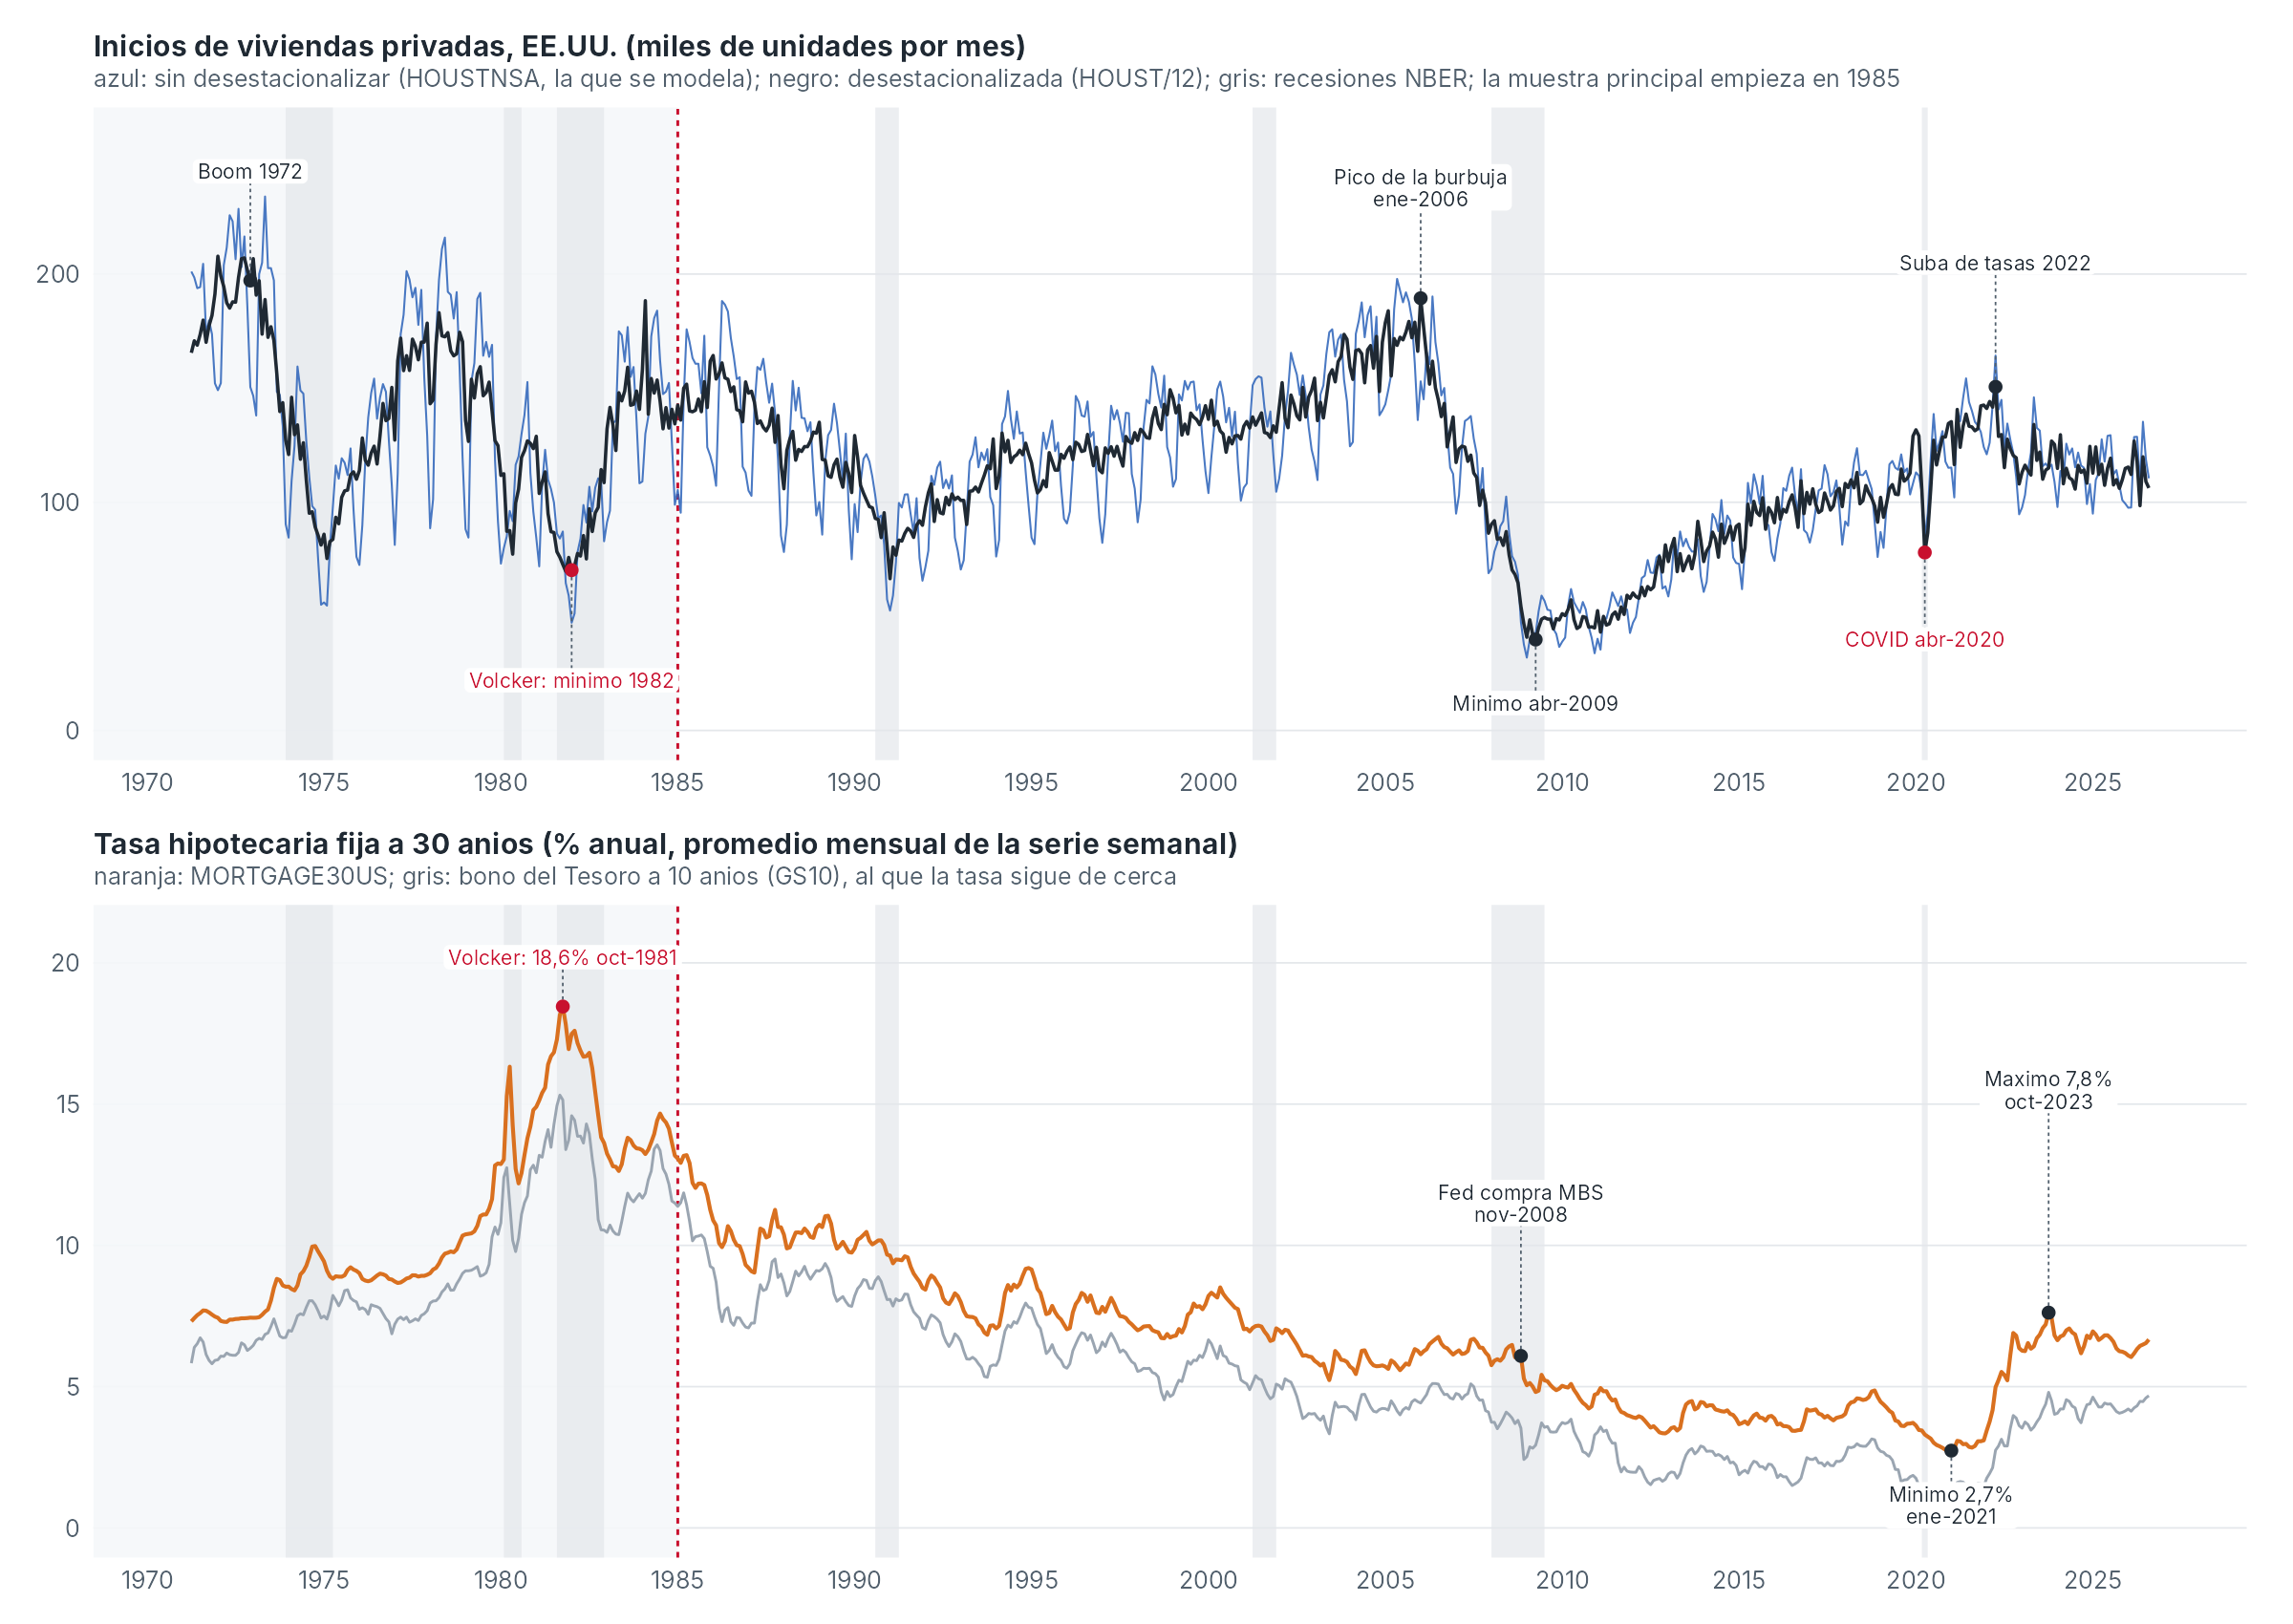
\includegraphics[width=\linewidth,height=0.90\textheight,keepaspectratio]{niveles_informe.png}
    \end{column}
    \begin{column}{0.28\textwidth}
      \small
      \begin{itemize}
        \item FRED: inicios (Census Bureau) y tasa a 30 años (Freddie Mac); 500 meses.
        \item Desde 1985: fuera el régimen Volcker.
        \item Ambas en $100\ln$: el logaritmo estabiliza la varianza y las diferencias se leen como variaciones \%.
        \item Sombreado: recesiones.
      \end{itemize}
    \end{column}
  \end{columns}
\end{frame}

% ---------- 4a. Estacionalidad [0:40] ----------
\begin{frame}
  \frametitle{Los inicios tienen una estacionalidad que cambia; la tasa no tiene}
  \centering\small
  \begin{tabular}{lccccc}
    \toprule
    Serie & Estac.\ fija & $p$ & $R^2$ binarias & Cambio de patrón & $p$ \\
    \midrule
    $\Delta\ln$ inicios & $F_{11,486}=43{,}5$ & $<0{,}001$ & 0,50 & \alert{$F_{11,475}=4{,}13$} & \alert{$<0{,}001$} \\
    $\Delta\ln$ tasa & \alert{$F_{11,486}=1{,}37$} & \alert{0,182} & 0,032 & $F_{11,475}=0{,}91$ & 0,532 \\
    \bottomrule
  \end{tabular}

  \smallskip
  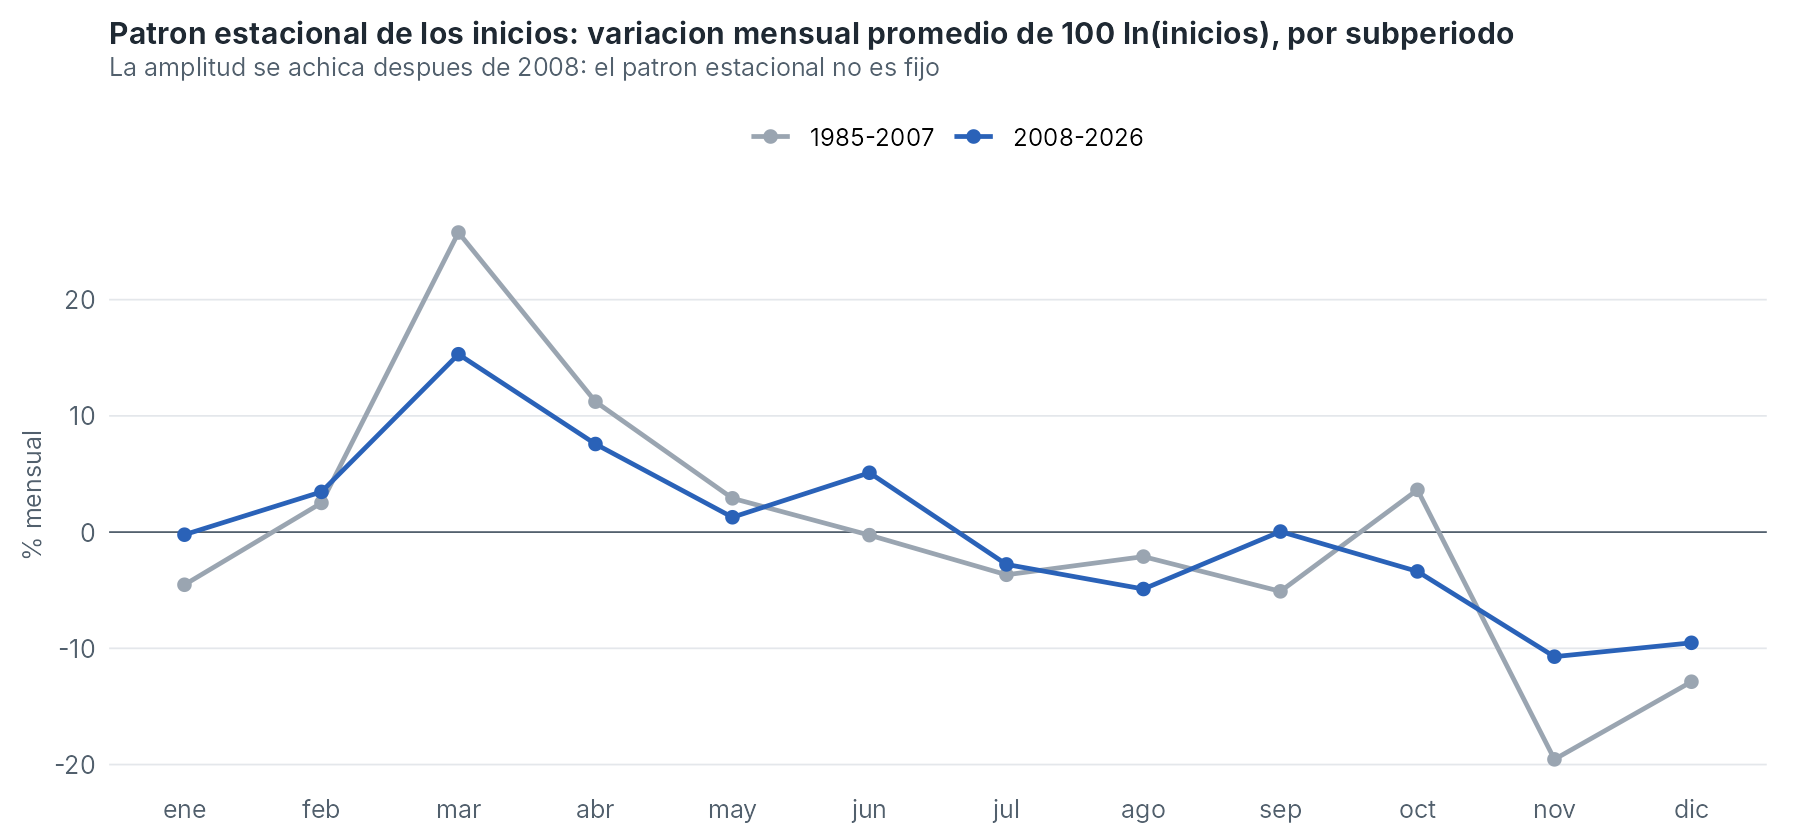
\includegraphics[width=0.80\linewidth,height=0.42\textheight,keepaspectratio]{estacionalidad_informe.png}

  \raggedright\footnotesize
  \begin{itemize}
    \item $\Delta$ de cada serie sobre 11 variables binarias mensuales; cambio de patrón: mes $\times$ subperíodo (1985--2007 vs.\ 2008--2026).
    \item Inicios: patrón que cambia $\Rightarrow$ estacionalidad estocástica $\Rightarrow$ $(1-B^{12})$. Tasa: sin estacionalidad.
  \end{itemize}
\end{frame}

% ---------- 4b0. Raiz unitaria [0:55] ----------
\begin{frame}
  \frametitle{Raíz unitaria: las dos series son $I(1)$; los inicios necesitan además $(1-B^{12})$}
  \footnotesize
  \textbf{ADF}, esquema descendente (Dickey y Pantula, 1987): primero se testea una segunda raíz sobre $\Delta$, después el nivel. 12 rezagos (sensibilidad con 24 y SBC); valores críticos de MacKinnon.
  \smallskip

  \centering
  \begin{tabular}{lcccc}
    \toprule
    & \multicolumn{2}{c}{Nivel ($H_0$: raíz unitaria)} & Primera diferencia & \\
    \cmidrule(lr){2-3}
    Serie & $\tau_\tau$ ($p$) & $\tau_\mu$ ($p$) & $\tau_\mu$ ($p$) & Orden \\
    \midrule
    $100\ln$ inicios & $-1{,}79$ (0,71) & $-1{,}86$ (0,35) & \alert{$-5{,}30$ ($<0{,}001$)} & $I(1)$ \\
    $100\ln$ tasa & $-1{,}96$ (0,62) & $-1{,}98$ (0,30) & \alert{$-5{,}66$ ($<0{,}001$)} & $I(1)$ \\
    \bottomrule
  \end{tabular}
  \raggedright
  \vspace{-1mm}
  \begin{itemize}\setlength{\itemsep}{0pt}
    \item En nivel no se rechaza la raíz unitaria (la tendencia no es significativa: se pasa a $\tau_\mu$). En la diferencia se rechaza $\Rightarrow$ \textbf{una diferencia regular}.
    \item El ADF solo testea la raíz en $z=1$: \textbf{no detecta la raíz estacional}. Sobre $(1-B^{12})x$ es frágil ($p=0{,}005$ con 12 rezagos; $0{,}055$ con SBC). Deciden el correlograma y el SBC:
  \end{itemize}
  \vspace{-1mm}
  \centering
  \begin{tabular}{lcc}
    \toprule
    Filtro de los inicios & Ljung--Box ($p$, 24) & $\Delta$SBC \\
    \midrule
    $(1-B)$ + binarias mensuales fijas & 0,39 & 49,1 \\
    $(1-B^{12})$ & 0,30 & 9,2 \\
    \alert{$(1-B)(1-B^{12})$} & \alert{0,47} & \alert{0,0} \\
    \bottomrule
  \end{tabular}
\end{frame}

% ---------- 4c. Modelo de lineas aereas [0:45] ----------
\begin{frame}
  \frametitle{El modelo de líneas aéreas: un MA restringido}
  \footnotesize
  ARIMA$(0,1,1)(0,1,1)_{12}$ (Box et al., 2015, cap.~9):
  \[ (1-B)(1-B^{12})\,x_t=(1-\theta B)(1-\Theta B^{12})\,a_t \]
  \begin{columns}[T]
    \begin{column}{0.50\textwidth}
      \textbf{Los dos filtros}
      \begin{itemize}
        \item $(1-B)$: saca la tendencia (raíz unitaria regular).
        \item $(1-B^{12})$: compara cada mes con el mismo mes del año anterior (estacionalidad que cambia).
      \end{itemize}
      \textbf{La parte MA, desarrollada}
      \[ (1-\theta B)(1-\Theta B^{12})=1-\theta B-\Theta B^{12}+\theta\Theta B^{13} \]
      MA(13) con coeficientes 2 a 11 nulos y el de $B^{13}$ restringido: 2 parámetros, no 13.
    \end{column}
    \begin{column}{0.48\textwidth}
      \textbf{Su FAC: solo rezagos 1, 11, 12 y 13}
      \[ \rho_1=\frac{-\theta}{1+\theta^2},\qquad \rho_{12}=\frac{-\Theta}{1+\Theta^2} \]
      \[ \rho_{11}=\rho_{13}=\frac{\theta\Theta}{(1+\theta^2)(1+\Theta^2)} \]
      Con $\hat\theta=0{,}46$ y $\hat\Theta=0{,}84$: $\rho_1\approx-0{,}38$, $\rho_{12}\approx-0{,}49$, $\rho_{11}=\rho_{13}\approx0{,}19$.

      \smallskip
      \alert{Es lo que muestra la FAC empírica de la filmina siguiente.}
    \end{column}
  \end{columns}
\end{frame}

% ---------- 4b. Cada serie [1:00] ----------
\begin{frame}
  \frametitle{Cada serie: dos diferencias para los inicios y un golpe transitorio en 2020}
  \begin{columns}[T]
    \begin{column}{0.49\textwidth}
      \centering
      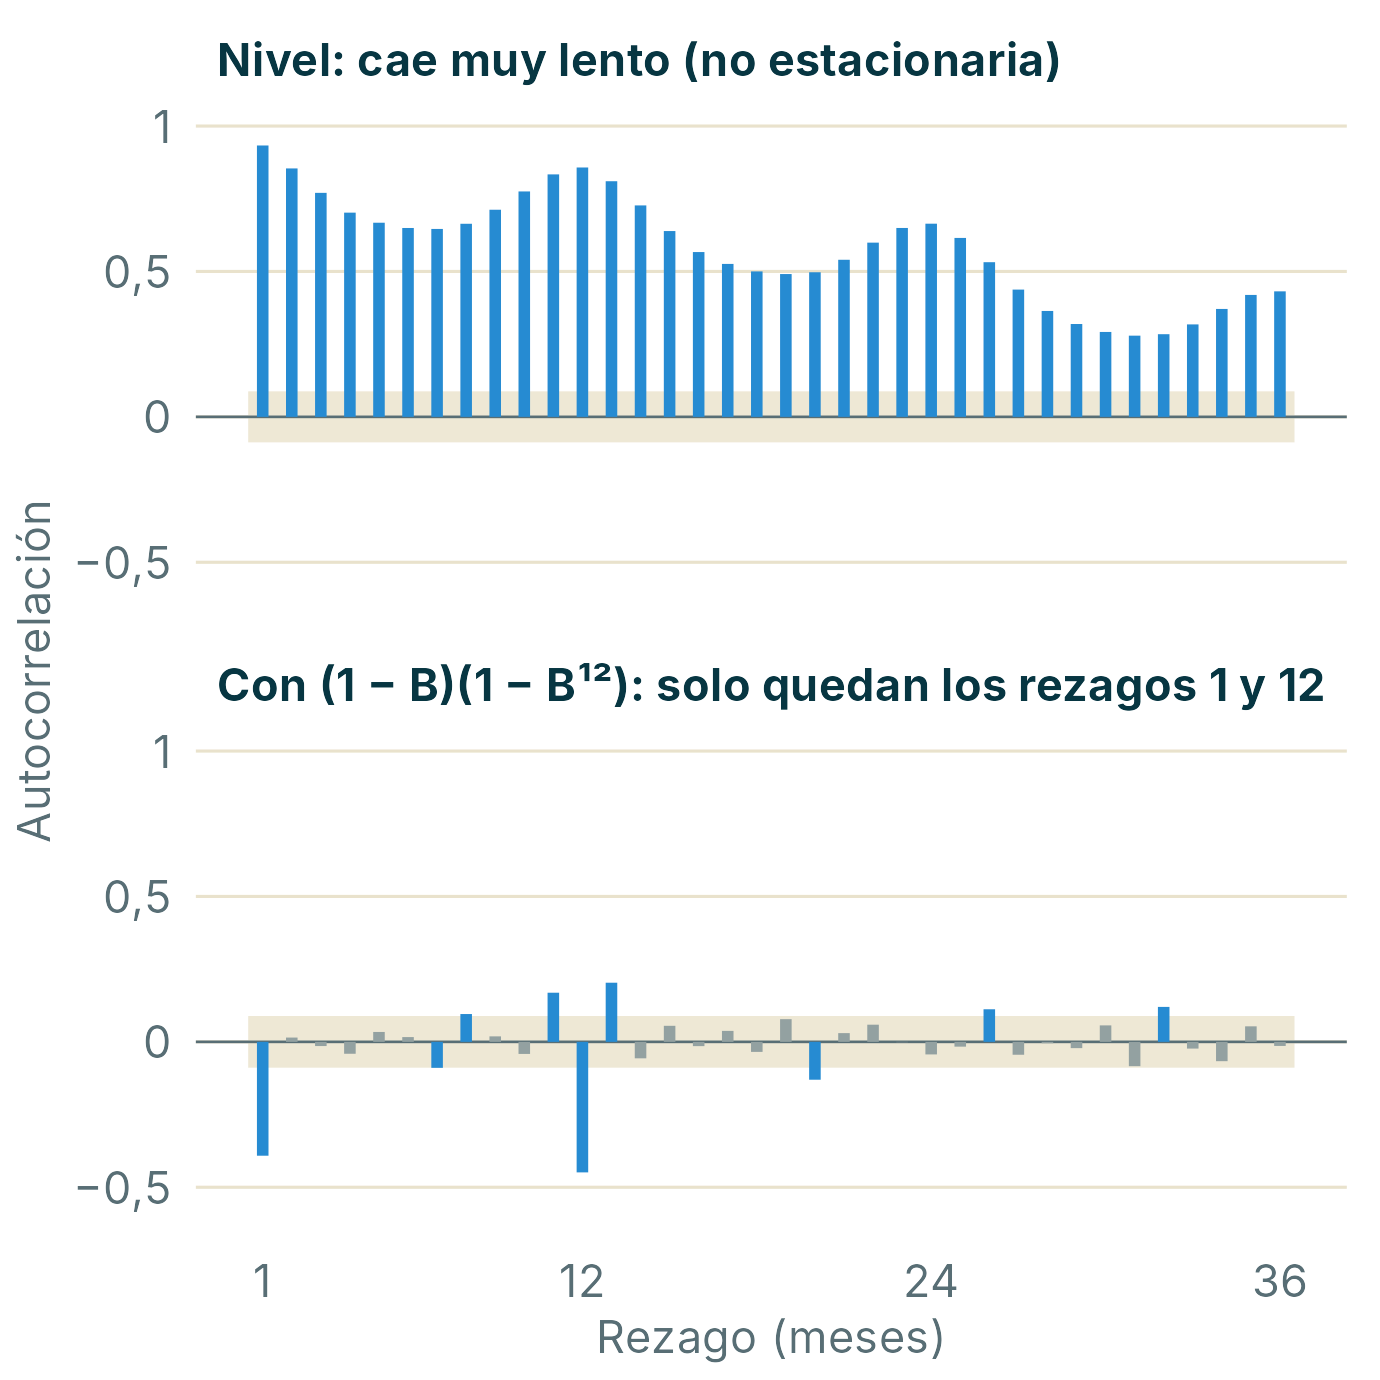
\includegraphics[width=\linewidth,height=0.52\textheight,keepaspectratio]{fac_inicios.png}

      \scriptsize
      \raggedright
      \textbf{Inicios}: líneas aéreas (Box et al., 2015, cap.~9), un MA(13) restringido:
      \[ (1-B)(1-B^{12})N_t=(1-\underset{(0{,}04)}{0{,}46}B)(1-\underset{(0{,}03)}{0{,}84}B^{12})\,a_t \]
      \textbf{Tasa}: $(1-B)\,y_t=(1+\underset{(0{,}04)}{0{,}44}B)\,a_t$
    \end{column}
    \begin{column}{0.49\textwidth}
      \centering
      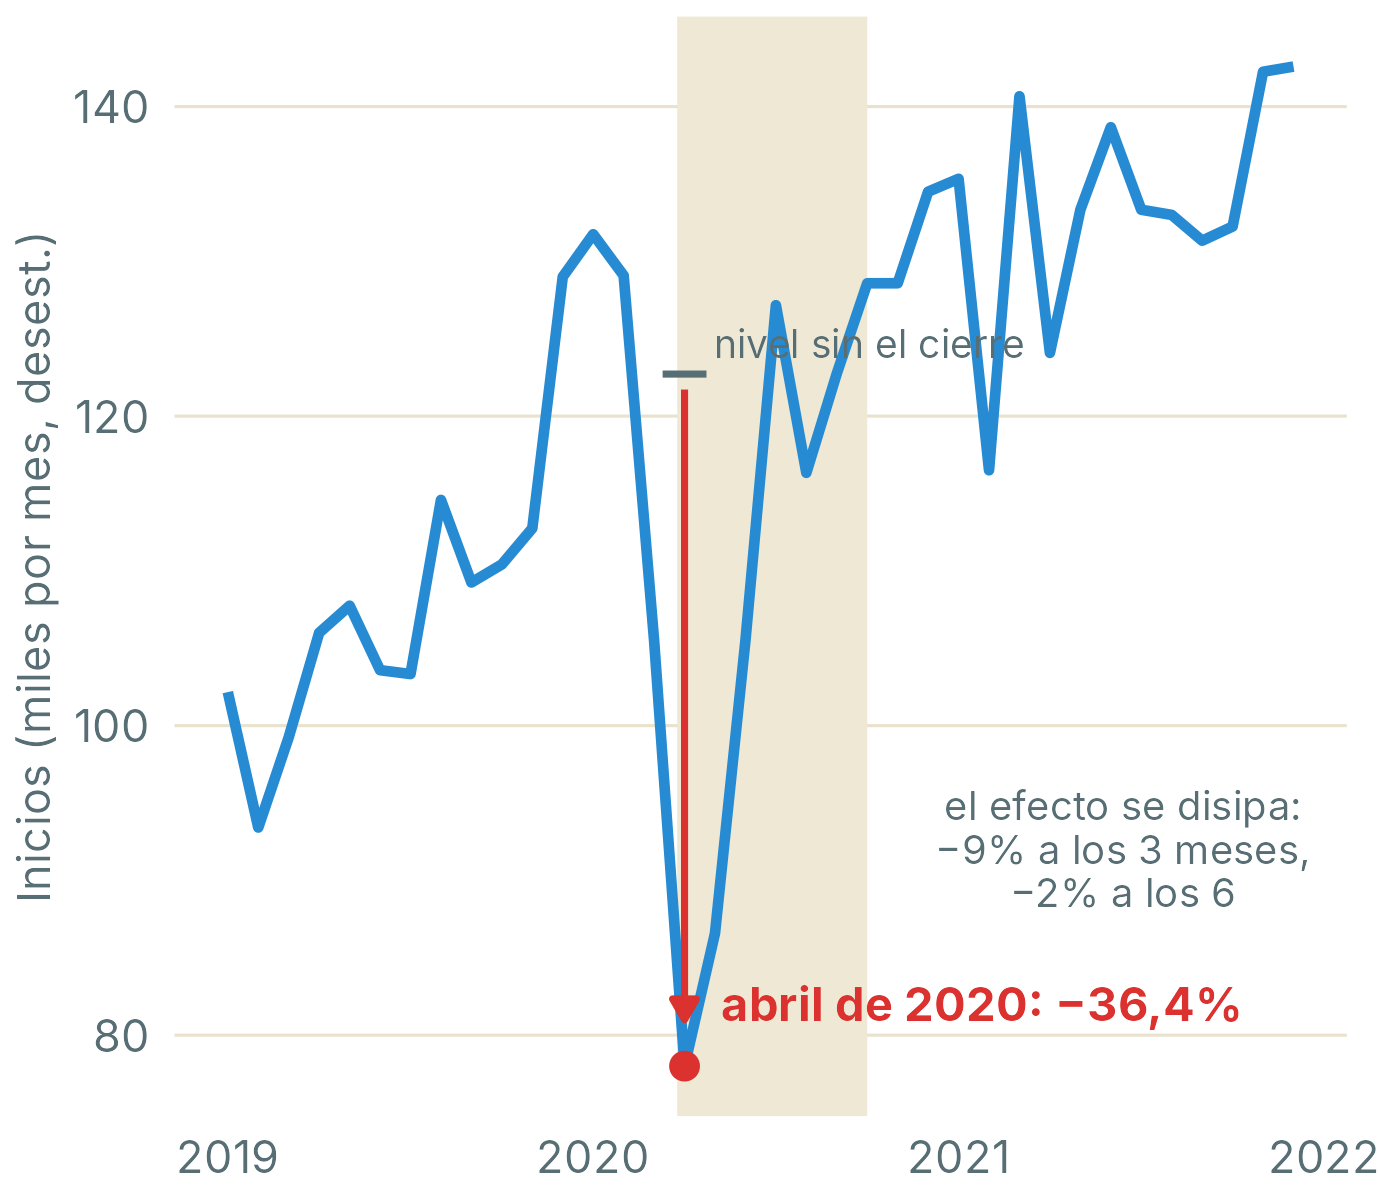
\includegraphics[width=\linewidth,height=0.52\textheight,keepaspectratio]{covid.png}

      \scriptsize
      \raggedright
      \textbf{COVID}: cambio transitorio en abril de 2020 ($-36{,}4\%$):
      \[ x_t=-\underset{(7{,}2)}{45{,}3}\,\frac{1}{1-0{,}60B}\,I_t^{2020.04}+N_t \]
    \end{column}
  \end{columns}
\end{frame}

% ---------- 5. Niveles [0:50] ----------
\section{Relación y exogeneidad}
\begin{frame}
  \frametitle{En niveles la relación es espuria y no hay cointegración}
  \begin{itemize}
    \item Regresión en niveles: pendiente \emph{positiva}, $R^2=0{,}26>DW=0{,}09$ $\Rightarrow$ espuria (Granger y Newbold, 1974).
  \end{itemize}
  \centering\small
  \begin{tabular}{llll}
    \toprule
    Prueba ($H_0$: no cointegración) & Estadístico & Valor crítico 5\% & Decisión \\
    \midrule
    Engle--Granger & $-3{,}00$ a $-1{,}78$ & $-3{,}35$ & No rechaza \\
    Johansen, traza ($K=3$) & 20,26 & 19,96 & Rechaza por poco \\
    Johansen, $\lambda_{\max}$ ($K=3$) & 15,34 & 15,67 & No rechaza \\
    Johansen sin variables COVID & 13,9 a 17,7 & 19,96 & No rechaza \\
    Bandas PSS, $F$ & 4,06 & 4,94 -- 5,73 & No rechaza \\
    \bottomrule
  \end{tabular}

  \raggedright
  \begin{itemize}
    \item El único rechazo es frágil y el vector no tiene sentido económico.
    \item $\Rightarrow$ \alert{Se trabaja en diferencias, sin modelo de corrección de errores.}
  \end{itemize}
\end{frame}

% ---------- 6. Exogeneidad [0:50] ----------
\begin{frame}
  \frametitle{Los inicios no anticipan a la tasa: se la puede tratar como exógena}
  \begin{columns}[T]
    \begin{column}{0.54\textwidth}
      \centering
      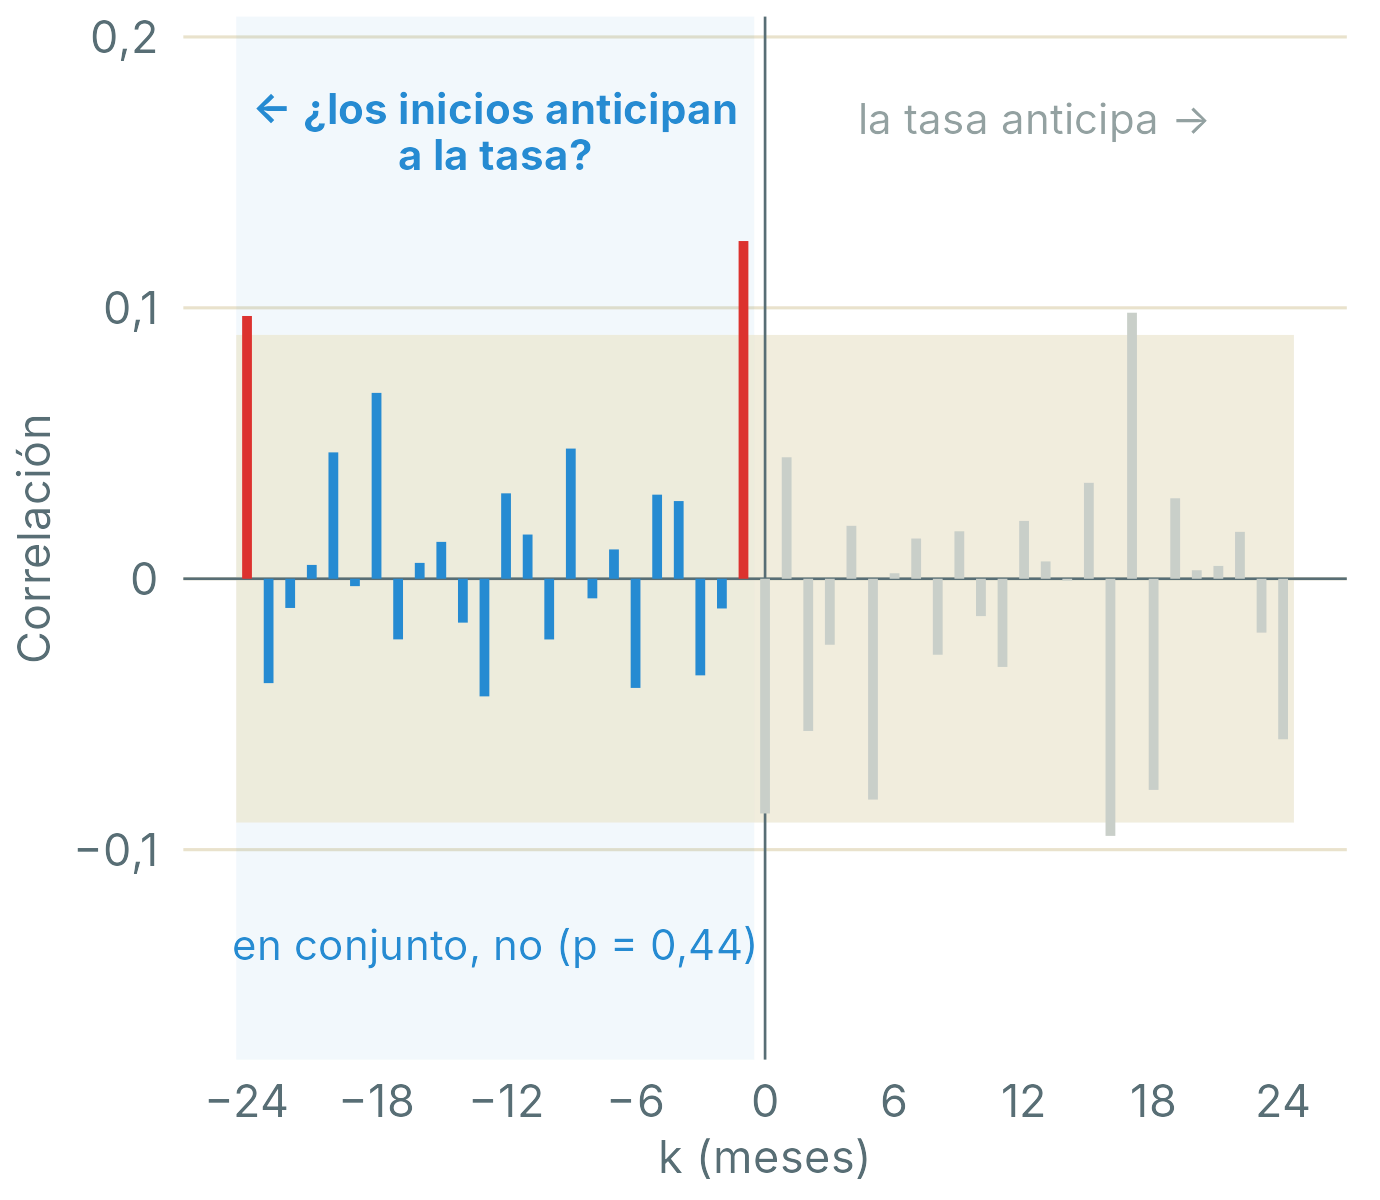
\includegraphics[width=\linewidth,height=0.80\textheight,keepaspectratio]{fcc_pre.png}
    \end{column}
    \begin{column}{0.44\textwidth}
      \small
      Tres contrastes del lado izquierdo ($k<0$):

      \smallskip
      \begin{tabular}{lc}
        \toprule
        Contraste & $p$ \\
        \midrule
        Innovaciones (Haugh) & 0,112 \\
        Preblanqueo & 0,438 \\
        Residuos vs.\ \emph{input} & 0,197 \\
        \bottomrule
      \end{tabular}

      \smallskip
      \begin{itemize}
        \item Ninguno rechaza. Queda una señal en $k=-1$: chica y positiva, la que predice la teoría.
        \item \alert{Función de transferencia} como modelo principal; VAR como control.
      \end{itemize}
    \end{column}
  \end{columns}
\end{frame}

% ---------- 7. Funcion de transferencia [1:15] ----------
\section{Función de transferencia}
\begin{frame}
  \frametitle{Una suba de 1 pp baja los inicios 6,3\%, con dos meses de retardo}
  \small
  \vspace{-3mm}
  \begin{gather*}
    Y_t=-\underset{(0{,}27)}{0{,}13}\;-\;\underset{(0{,}029)}{0{,}112}\,\frac{1}{1-0{,}75B}\,X_{t-2}\;-\;\underset{(5{,}5)}{43{,}8}\,TC_t+N_t\\[-1mm]
    (1-\underset{(0{,}02)}{0{,}97}B)(1-\underset{(0{,}11)}{0{,}52}B^{12})\,N_t=(1-\underset{(0{,}04)}{1{,}47}B+\underset{(0{,}04)}{0{,}52}B^2)(1-\underset{(0{,}09)}{0{,}74}B^{12})\,e_t,\qquad \hat\sigma_e=6{,}6
  \end{gather*}
  \vspace{-4mm}
  \begin{columns}[T]
    \begin{column}{0.54\textwidth}
      \centering
      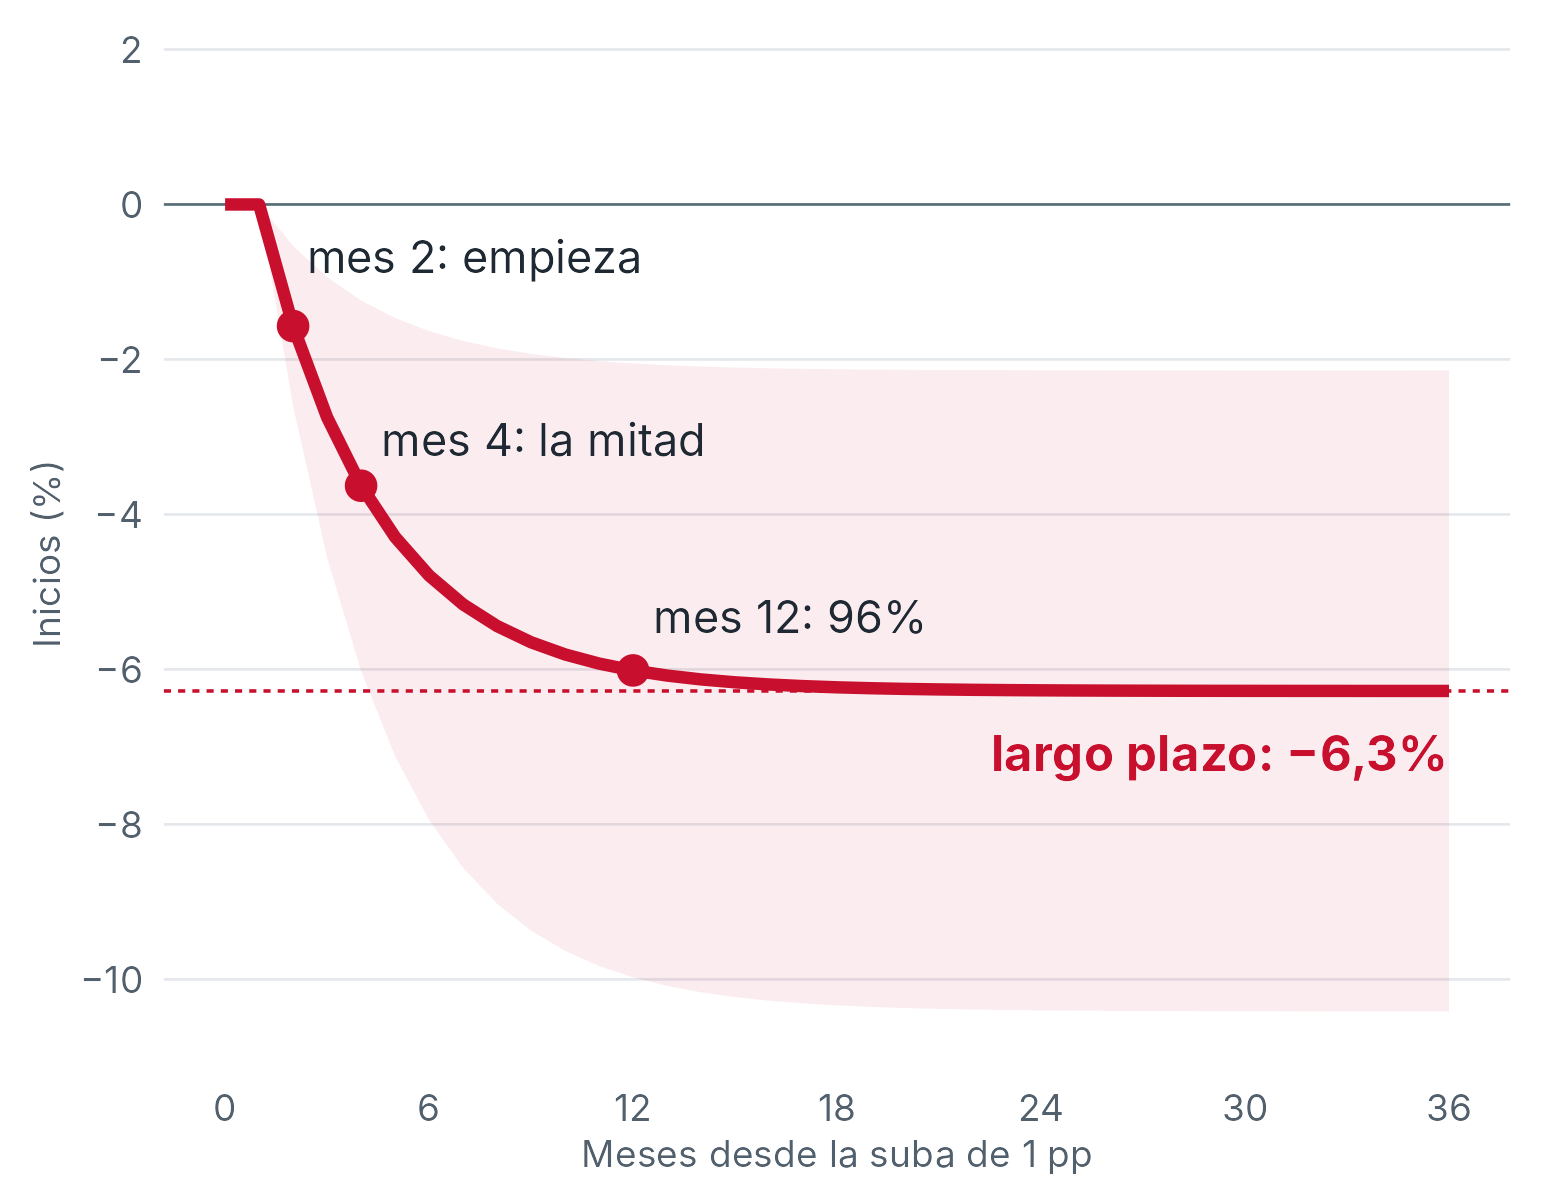
\includegraphics[width=\linewidth,height=0.50\textheight,keepaspectratio]{resp_ft.png}
    \end{column}
    \begin{column}{0.44\textwidth}
      \footnotesize
      \begin{itemize}
        \item $Y$, $X$: variación mensual de inicios (desestacionalizados) y tasa ($100\ln$).
        \item $\delta_0=-0{,}112$, $\phi=0{,}75$: ganancia $g=\delta_0/(1-\phi)=-0{,}45$ (e.e.\ 0,15).
        \item La curva es la respuesta acumulada ante $+1$ pp (evaluada a la tasa de 6,67\%); la banda, su intervalo de 95\%.
      \end{itemize}
    \end{column}
  \end{columns}
  \vfill
  {\scriptsize Inicios desestacionalizados por el Census (X-13ARIMA-SEATS); los términos estacionales del ruido recogen la estacionalidad residual. Errores estándar entre paréntesis.\par}
\end{frame}

% ---------- 8. Robustez [1:10] ----------
\section{Robustez}
\begin{frame}
  \frametitle{Robusto: sin suponer exogeneidad, con otros modelos y en otros períodos}
  \begin{columns}[T]
    \begin{column}{0.49\textwidth}
      \centering
      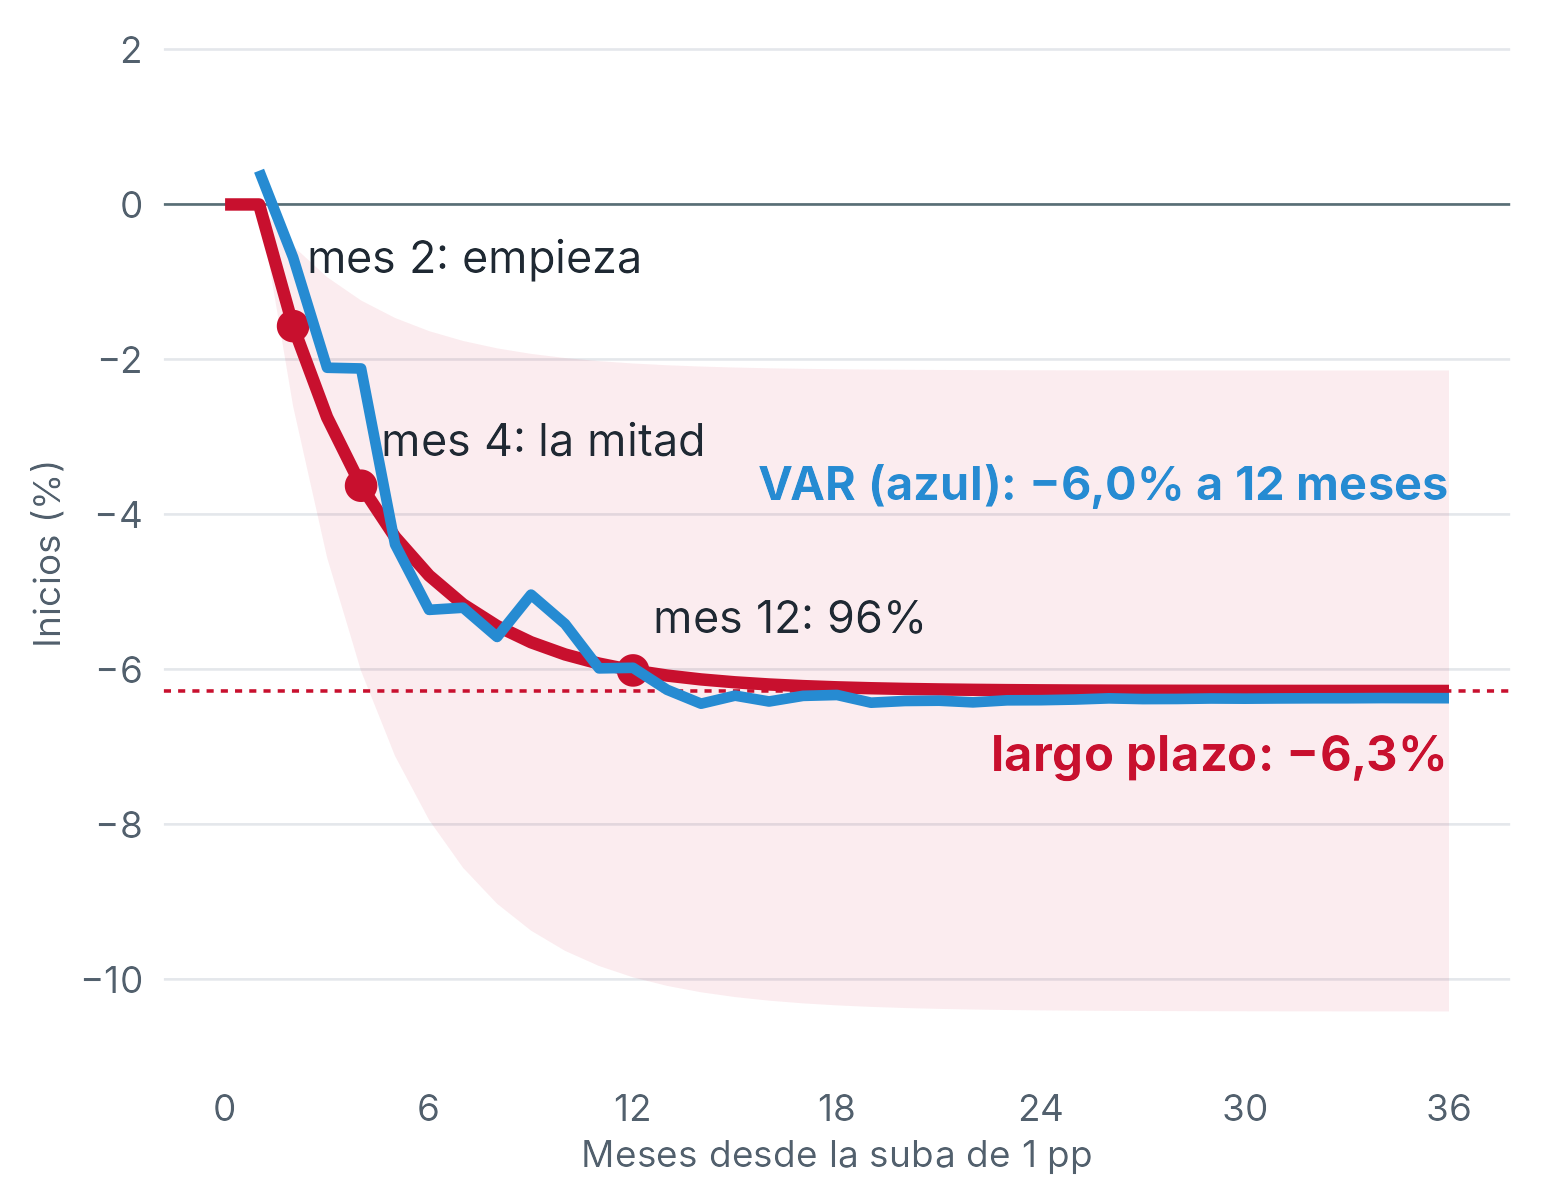
\includegraphics[width=\linewidth,height=0.56\textheight,keepaspectratio]{resp_ft_var.png}
    \end{column}
    \begin{column}{0.49\textwidth}
      \centering
      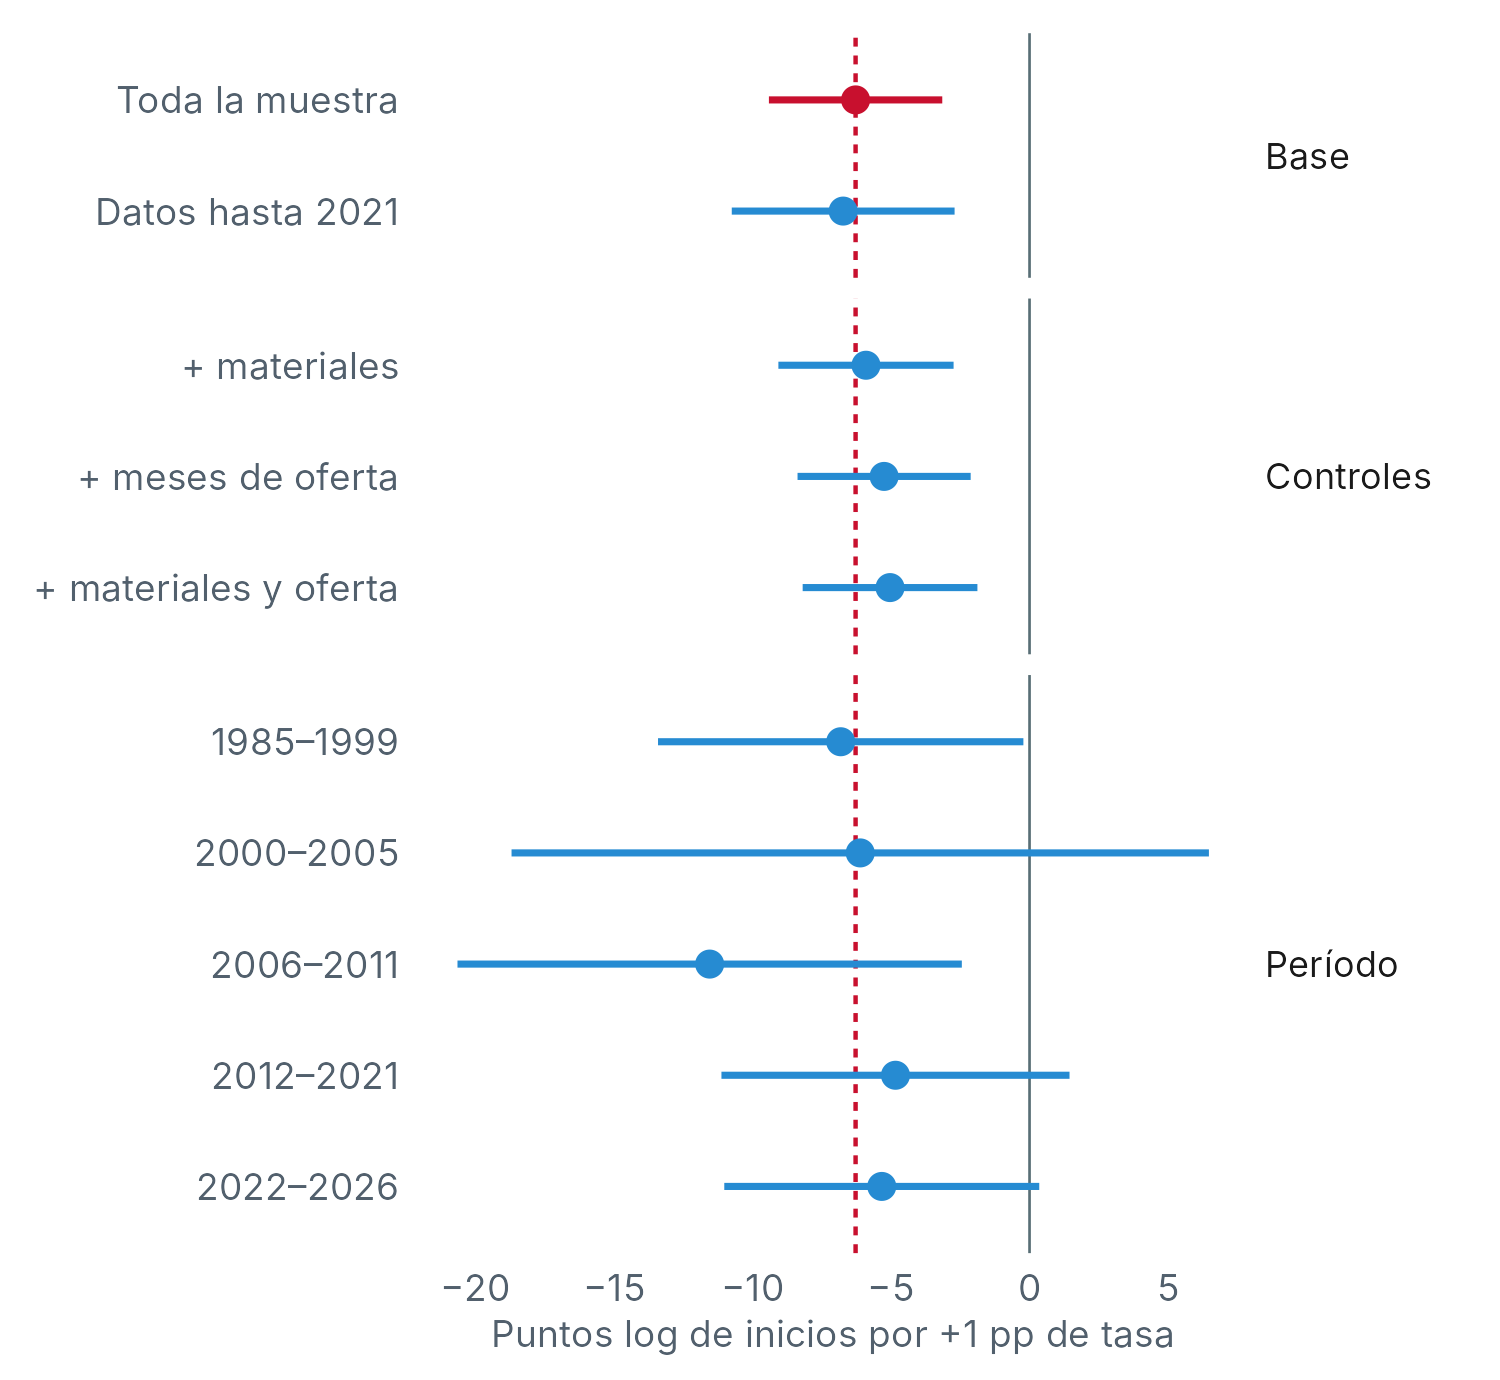
\includegraphics[width=\linewidth,height=0.56\textheight,keepaspectratio]{estab_especif.png}
    \end{column}
  \end{columns}
  \small
  \begin{itemize}
    \item VAR(9) con las dos variables endógenas, $z_t=(X_t,Y_t)'$: $\;z_t=c+\sum_{i=1}^{9}A_i\,z_{t-i}+\gamma\,TC_t+u_t$, Cholesky con la tasa primero. \alert{$-6{,}0\%$} a 12 meses; la retroalimentación es chica (tasa $+1{,}3\%$ ante un shock de inicios).
    \item Costos, oferta y subperíodos: igual efecto ($p=0{,}81$; sin quiebre en 2022). Con el bono, $-6{,}5\%$; permisos, un mes antes ($-8{,}0\%$).
  \end{itemize}
\end{frame}

% ---------- 9. Episodio [1:00] ----------
\section{El episodio 2022--2024}
\begin{frame}
  \frametitle{En 2022--2024 el modelo predijo más caída de la que hubo}
  \centering
  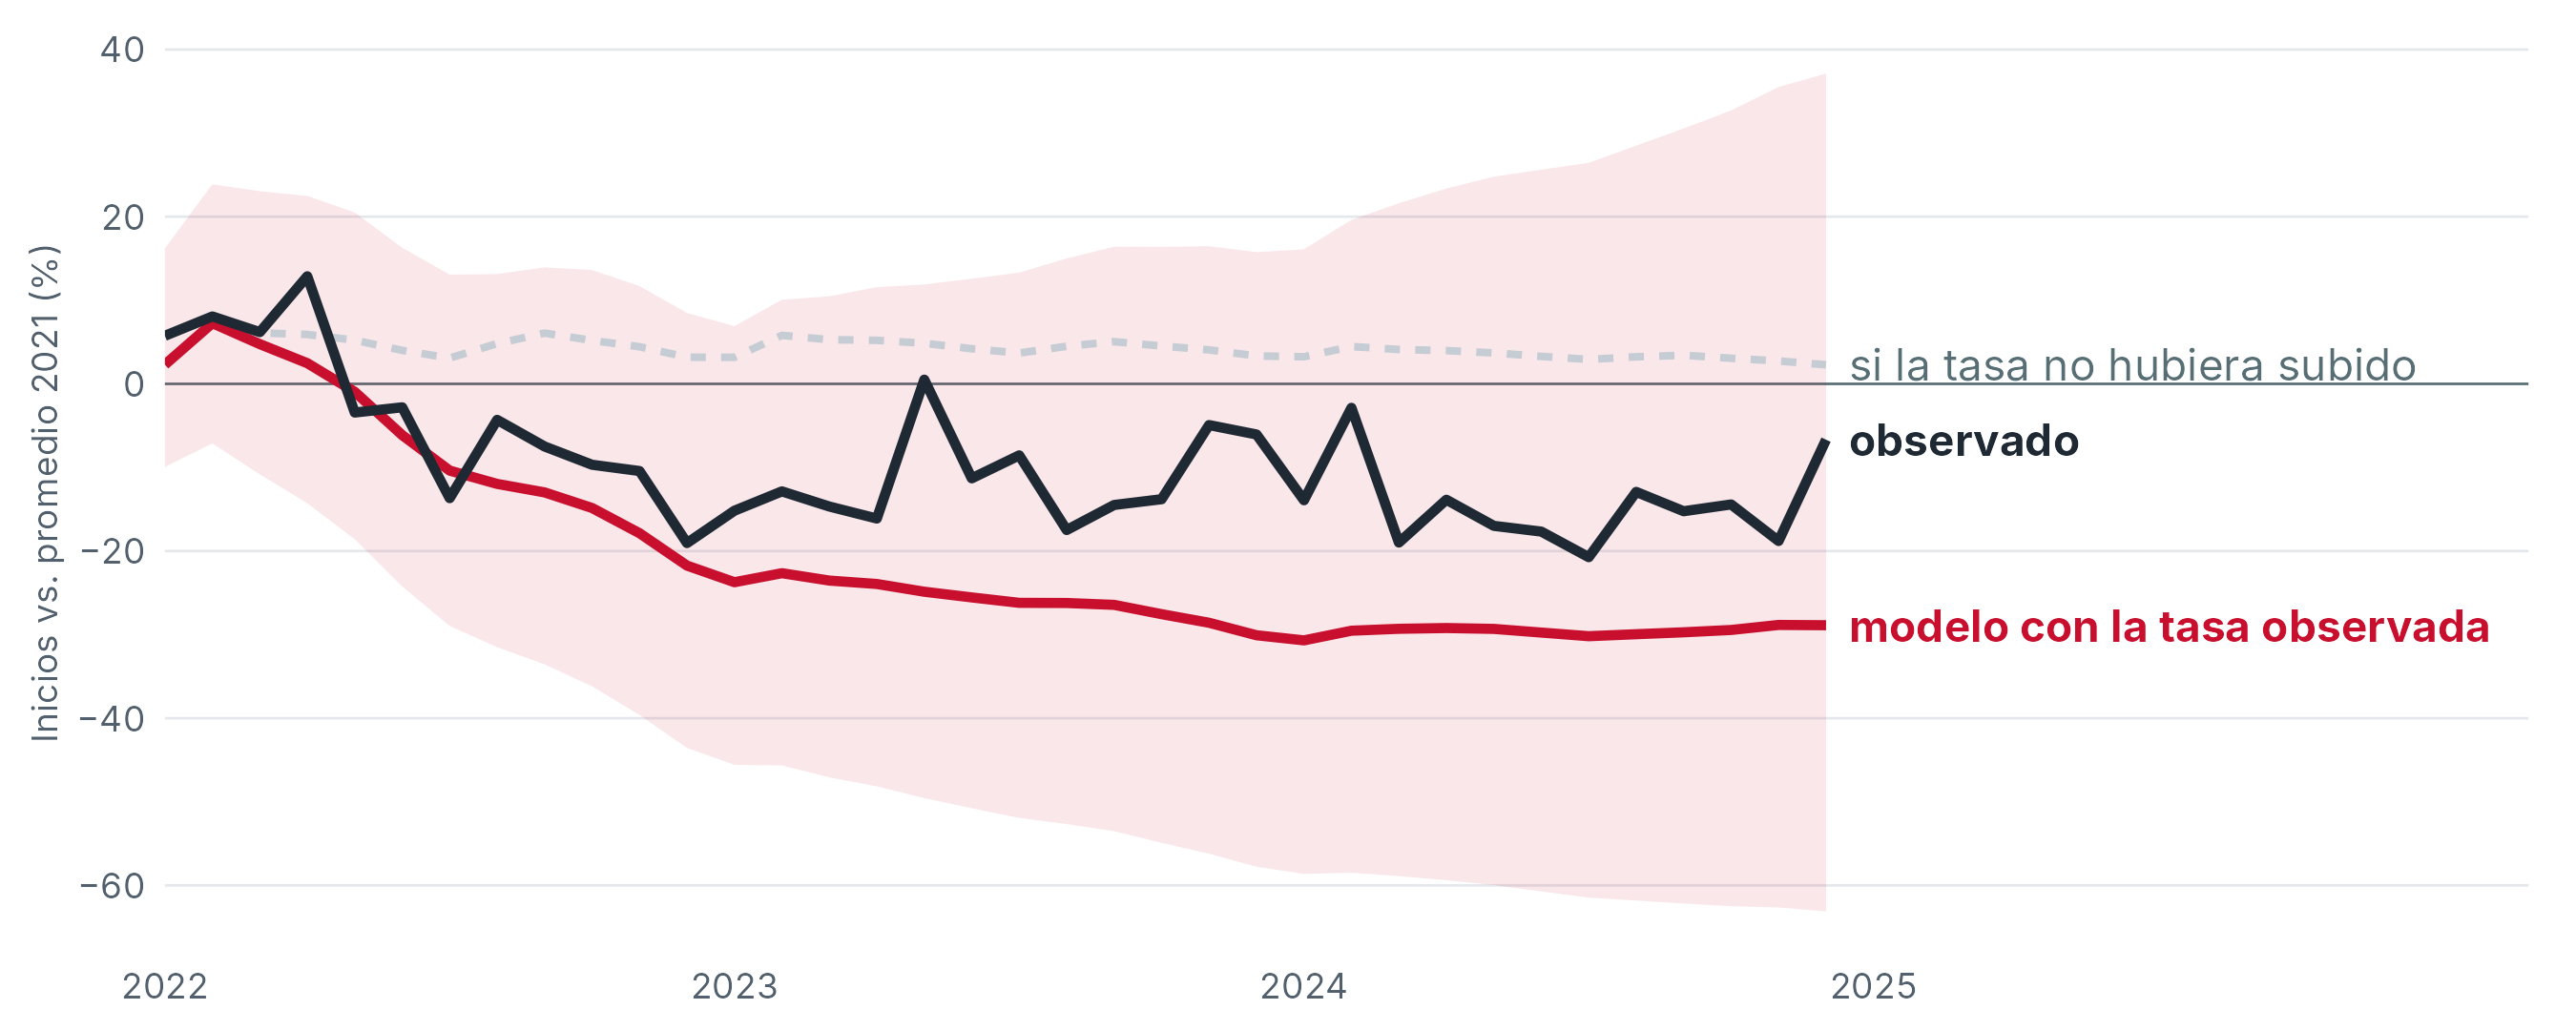
\includegraphics[width=\linewidth,height=0.62\textheight,keepaspectratio]{episodio.png}

  \raggedright\small
  \begin{itemize}
    \item Modelo estimado \alert{solo con datos hasta diciembre de 2021} y alimentado con la tasa observada.
    \item Acierta la dirección y el momento. Pero atribuye a la tasa una caída de 31,9\% en 2024, contra 14,6\% observado.
  \end{itemize}
\end{frame}

% ---------- 10. Descomposicion [1:00] ----------
\begin{frame}
  \frametitle{La tasa restó 38 puntos; otros factores devolvieron 19}
  \begin{columns}[T]
    \begin{column}{0.50\textwidth}
      \centering
      % Cascada 2024 vs. 2021 (puntos log); 1 unidad = 0,115 cm
      \begin{tikzpicture}[y=0.115cm, x=0.88cm, font=\scriptsize]
        \foreach \v in {-40,-30,-20,-10,0} {
          \draw[gReja] (-0.35,\v) -- (6.75,\v);
          \node[anchor=east, text=gSec] at (-0.4,\v) {\v};
        }
        \node[rotate=90, text=gSec] at (-1.5,-17) {puntos log, 2024 vs.\ 2021};
        \draw[gSec, thick] (-0.35,0) -- (6.75,0);
        % barras: inicio, fin
        \fill[gGris] (0,0) rectangle (1.2,3.3);
        \fill[gRojo] (1.8,3.3) rectangle (3.0,-35.1);
        \fill[gAzul] (3.6,-35.1) rectangle (4.8,-15.8);
        \fill[gTinta] (5.4,0) rectangle (6.6,-15.7);
        % conectores
        \draw[gSec, densely dashed] (1.2,3.3) -- (1.8,3.3);
        \draw[gSec, densely dashed] (3.0,-35.1) -- (3.6,-35.1);
        \draw[gSec, densely dashed] (4.8,-15.8) -- (5.4,-15.8);
        % valores
        \node[above, text=gSec, font=\footnotesize\bfseries] at (0.6,3.3) {$+3{,}3$};
        \node[below, text=gRojo, font=\footnotesize\bfseries] at (2.4,-35.1) {$-38{,}4$};
        \node[above, text=gAzul, font=\footnotesize\bfseries] at (4.2,-15.8) {$+19{,}3$};
        \node[below, text=gTinta, font=\footnotesize\bfseries] at (6.0,-15.7) {$-15{,}7$};
        % categorias
        \foreach \x/\t in {0.6/{Sin cambios\\de tasa}, 2.4/{Tasa}, 4.2/{Otros\\factores}, 6.0/{Observado}}
          \node[align=center, text=gTinta, anchor=north] at (\x,-41.5) {\t};
      \end{tikzpicture}

      \vspace{1mm}
      {\tiny\color{gSec} Cada barra parte de donde terminó la anterior; la observada, desde cero. Por redondeo, $3{,}3-38{,}4+19{,}3=-15{,}8$.\par}
    \end{column}
    \begin{column}{0.48\textwidth}
      \small
      \begin{itemize}
        \item La tasa explica la dirección de la caída; otros factores compensaron la mitad.
        \item \alert{No hay quiebre:} el error a 36 meses es de 0,8 desvíos y los errores a un paso no tienen sesgo ($p=0{,}54$).
        \item Cuidado: $\phi$ está poco identificado antes de 2022.
        \item Asimetría y \emph{lock-in}: indicios dentro de la muestra, sin respaldo fuera.
      \end{itemize}
    \end{column}
  \end{columns}
\end{frame}

% ---------- 11. Conclusiones [0:50] ----------
\section{Conclusiones}
\begin{frame}
  \frametitle{Conclusiones}
  \begin{block}{¿Qué se encuentra?}
    \begin{itemize}
      \item $+1$ pp de tasa $\Rightarrow$ inicios $\approx -6\%$: empieza a los 2 meses, mitad a los 4, casi todo en un año.
      \item Robusto a VAR, bono, permisos, costos y oferta, y subperíodos.
      \item Sin relación de largo plazo en niveles; retroalimentación chica.
      \item 2022--2024: la tasa explica la caída; el resto, perturbaciones de tamaño normal.
    \end{itemize}
  \end{block}
  \begin{alertblock}{Límites y extensiones}
    \small $\phi$ poco identificado antes de 2022; varianza no constante; VAR sensible a los rezagos. Pendiente: canal de precios, tipos de vivienda y \emph{lock-in} con la tasa media efectiva.
  \end{alertblock}
\end{frame}

% ---------- Referencias ----------
\begin{frame}[allowframebreaks]
  \frametitle{Referencias}
  \footnotesize
  \begin{thebibliography}{99}
    \bibitem{r0} Box, G., Jenkins, G., Reinsel, G. y Ljung, G. (2015). \emph{Time Series Analysis: Forecasting and Control} (5.ª ed.). Wiley.
    \bibitem{r1} Brown, R. L., Durbin, J. y Evans, J. M. (1975). Techniques for testing the constancy of regression relationships over time. \emph{Journal of the Royal Statistical Society, Series B}, 37(2), 149--192.
    \bibitem{r2} Chow, G. C. (1960). Tests of equality between sets of coefficients in two linear regressions. \emph{Econometrica}, 28(3), 591--605.
    \bibitem{r3} Dickey, D. A. y Pantula, S. G. (1987). Determining the order of differencing in autoregressive processes. \emph{Journal of Business \& Economic Statistics}, 5(4), 455--461.
    \bibitem{r4} Enders, W. (2015). \emph{Applied Econometric Time Series} (4.ª ed.). Wiley.
    \bibitem{r5} Ferreira, F., Gyourko, J. y Tracy, J. (2010). Housing busts and household mobility. \emph{Journal of Urban Economics}, 68(1), 34--45.
    \bibitem{r6} Gonçalves, S. y Kilian, L. (2004). Bootstrapping autoregressions with conditional heteroskedasticity of unknown form. \emph{Journal of Econometrics}, 123(1), 89--120.
    \bibitem{r7} Granger, C. W. J. y Lee, T.-H. (1989). Investigation of production, sales and inventory relationships using multicointegration and non-symmetric error correction models. \emph{Journal of Applied Econometrics}, 4(S1), S145--S159.
    \bibitem{r8} Granger, C. W. J. y Newbold, P. (1974). Spurious regressions in econometrics. \emph{Journal of Econometrics}, 2(2), 111--120.
    \bibitem{r9} Greene, W. H. (2018). \emph{Econometric Analysis} (8.ª ed.). Pearson.
    \bibitem{r10} Hallin, M., La Vecchia, D. y Liu, H. (2022). Center-outward R-estimation for semiparametric VARMA models. \emph{Journal of the American Statistical Association}, 117(538), 925--938.
    \bibitem{r11} Haugh, L. D. (1976). Checking the independence of two covariance-stationary time series: a univariate residual cross-correlation approach. \emph{Journal of the American Statistical Association}, 71(354), 378--385.
    \bibitem{r12} Hosking, J. R. M. (1980). The multivariate portmanteau statistic. \emph{Journal of the American Statistical Association}, 75, 602--608.
    \bibitem{r13} MacKinnon, J. G. (2010). Critical values for cointegration tests. Queen\textquotesingle s Economics Department Working Paper 1227.
    \bibitem{r14} Mayer, C. J. y Somerville, C. T. (2000). Residential construction: using the urban growth model to estimate housing supply. \emph{Journal of Urban Economics}, 48(1), 85--109.
    \bibitem{r15} Pesaran, M. H., Shin, Y. y Smith, R. J. (2001). Bounds testing approaches to the analysis of level relationships. \emph{Journal of Applied Econometrics}, 16(3), 289--326.
    \bibitem{r16} Poterba, J. M. (1984). Tax subsidies to owner-occupied housing: an asset-market approach. \emph{Quarterly Journal of Economics}, 99(4), 729--752.
    \bibitem{r17} Quigley, J. M. (1987). Interest rate variations, mortgage prepayments and household mobility. \emph{Review of Economics and Statistics}, 69(4), 636--643.
    \bibitem{r18} Sims, C. A. (1980). Macroeconomics and reality. \emph{Econometrica}, 48(1), 1--48.
    \bibitem{r19} Topel, R. y Rosen, S. (1988). Housing investment in the United States. \emph{Journal of Political Economy}, 96(4), 718--740.
    \bibitem{r20} U.S. Census Bureau (2017). \emph{X-13ARIMA-SEATS Reference Manual}, versión 1.1. Washington, DC.
  \end{thebibliography}
\end{frame}

% ============ Respaldo (para preguntas) ============
\appendix
\section*{Respaldo}

\begin{frame}
  \frametitle{Respaldo: FAC de los inicios con cada filtro}
  \centering
  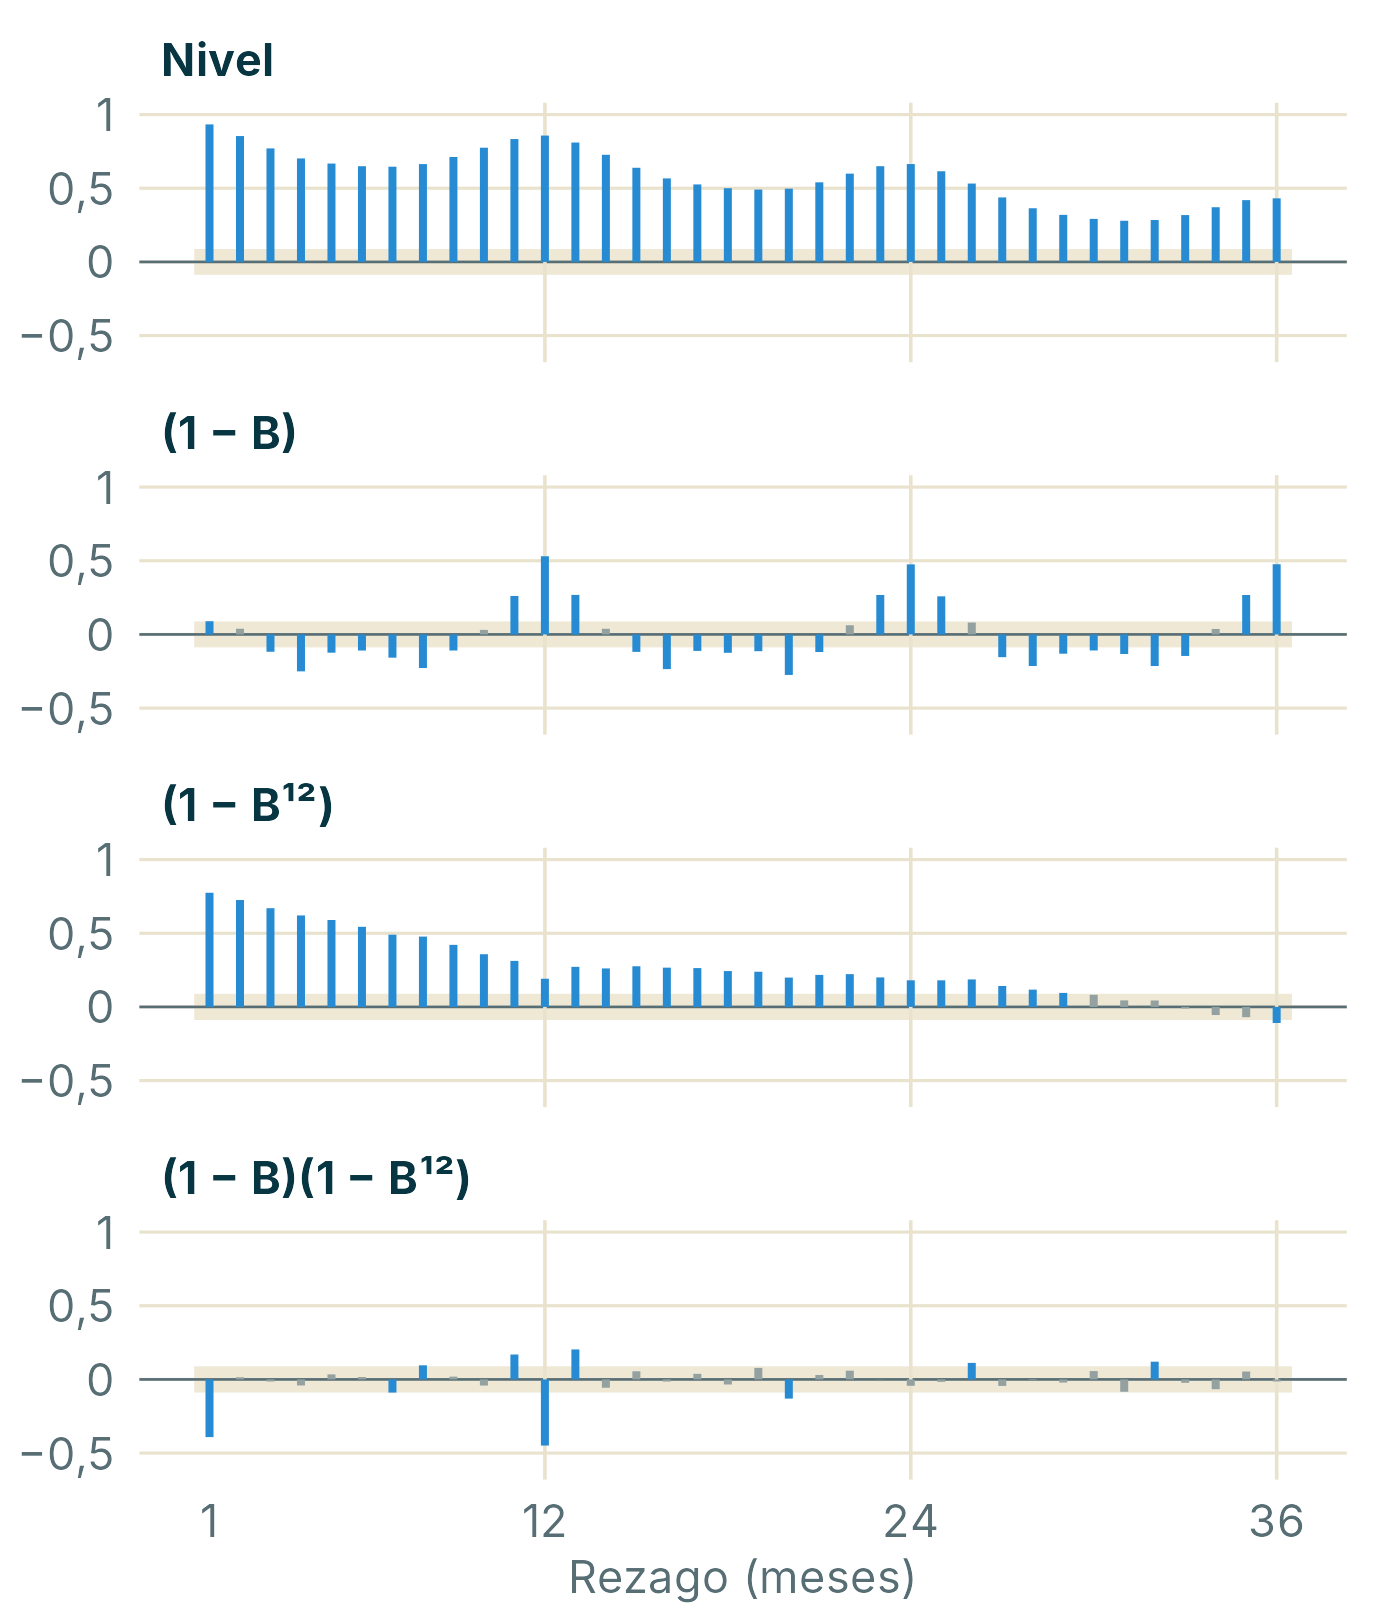
\includegraphics[width=\linewidth,height=0.78\textheight,keepaspectratio]{fac_inicios_4.png}
\end{frame}

\begin{frame}
  \frametitle{Respaldo: las tres formas de la intervención}
  \begin{columns}[T]
    \begin{column}{0.55\textwidth}
      \centering
      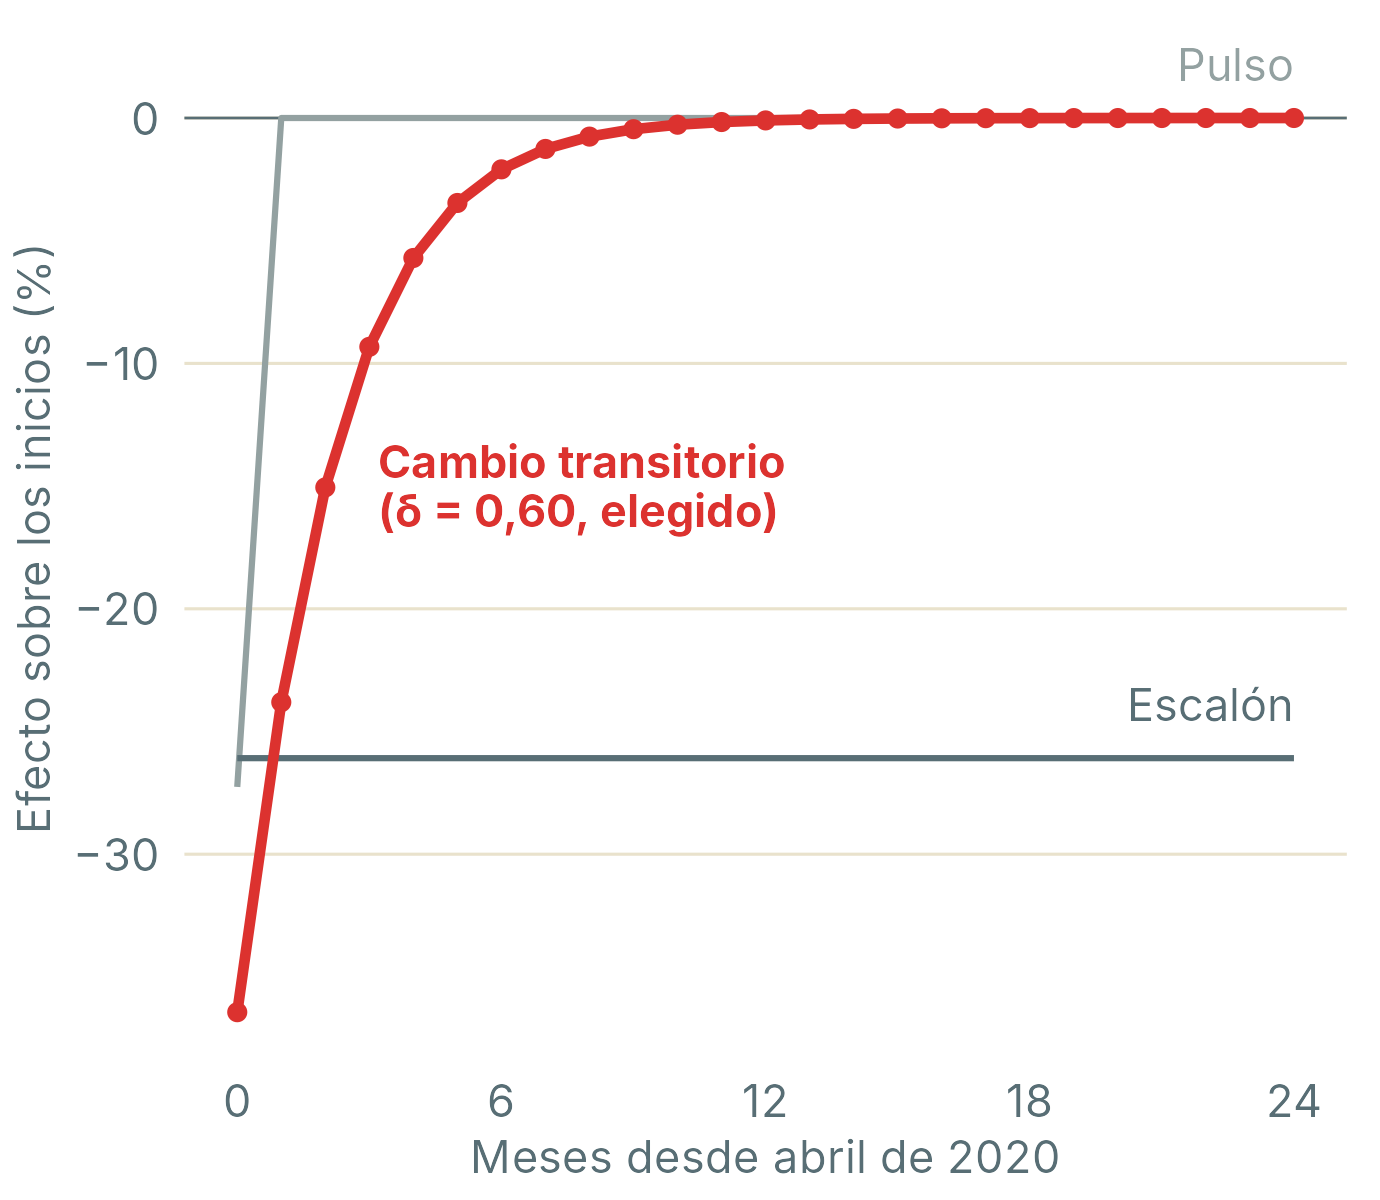
\includegraphics[width=\linewidth,height=0.80\textheight,keepaspectratio]{intervencion.png}
    \end{column}
    \begin{column}{0.43\textwidth}
      \small
      \begin{itemize}
        \item Pulso: $\xi(B)=1$. Transitoria: $\xi(B)=1/(1-\delta B)$. Escalón: $\xi(B)=1/(1-B)$.
        \item $\delta$ por perfil de verosimilitud; forma por SBC.
        \item La transitoria gana por 10,1 puntos al pulso y por 14,3 al escalón.
      \end{itemize}
    \end{column}
  \end{columns}
\end{frame}

\begin{frame}
  \frametitle{Respaldo: pesos de la respuesta al impulso}
  \begin{columns}[T]
    \begin{column}{0.55\textwidth}
      \centering
      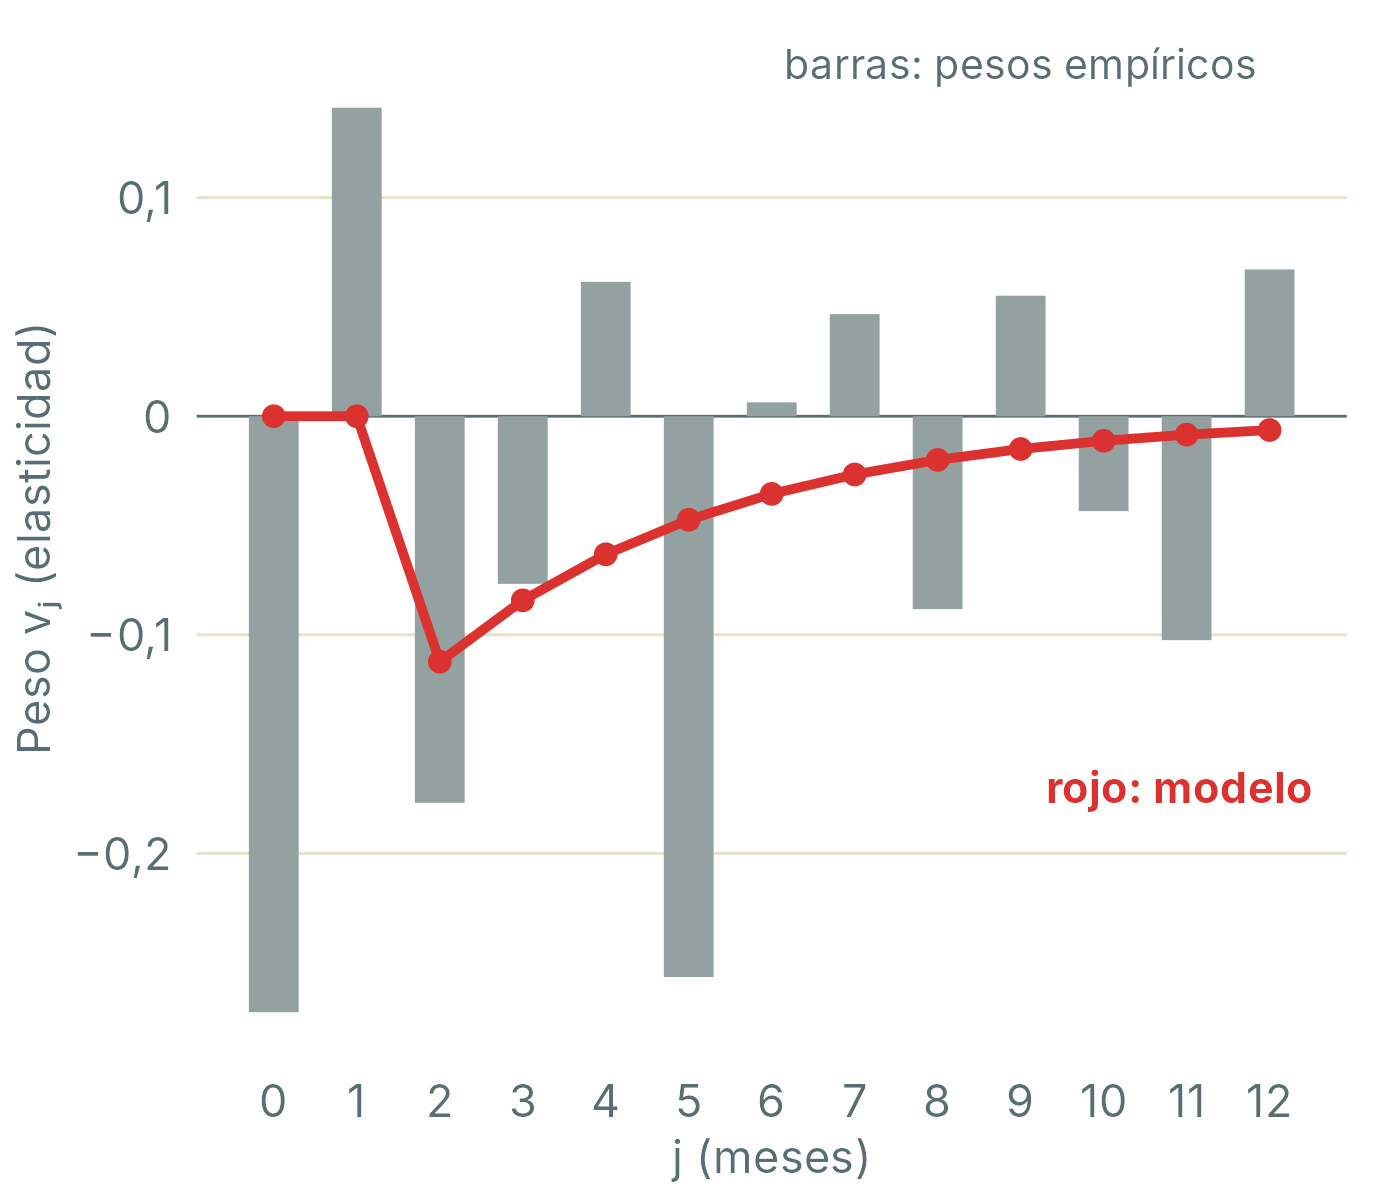
\includegraphics[width=\linewidth,height=0.80\textheight,keepaspectratio]{pesos.png}
    \end{column}
    \begin{column}{0.43\textwidth}
      \small
      \begin{itemize}
        \item Barras: pesos empíricos de la correlación cruzada preblanqueada. Rojo: $v_j=\delta_0\phi^{\,j-2}$.
        \item Sin picos nítidos ($p=0{,}57$): la forma se eligió comparando modelos por SBC.
        \item Con otros ruidos la ganancia va de $-4{,}8$ a $-6{,}3\%$ por pp.
      \end{itemize}
    \end{column}
  \end{columns}
\end{frame}

\begin{frame}
  \frametitle{Respaldo: el VAR en desvíos y su sensibilidad}
  \begin{columns}[T]
    \begin{column}{0.49\textwidth}
      \centering
      {\small Inicios ante un shock de tasa}\\
      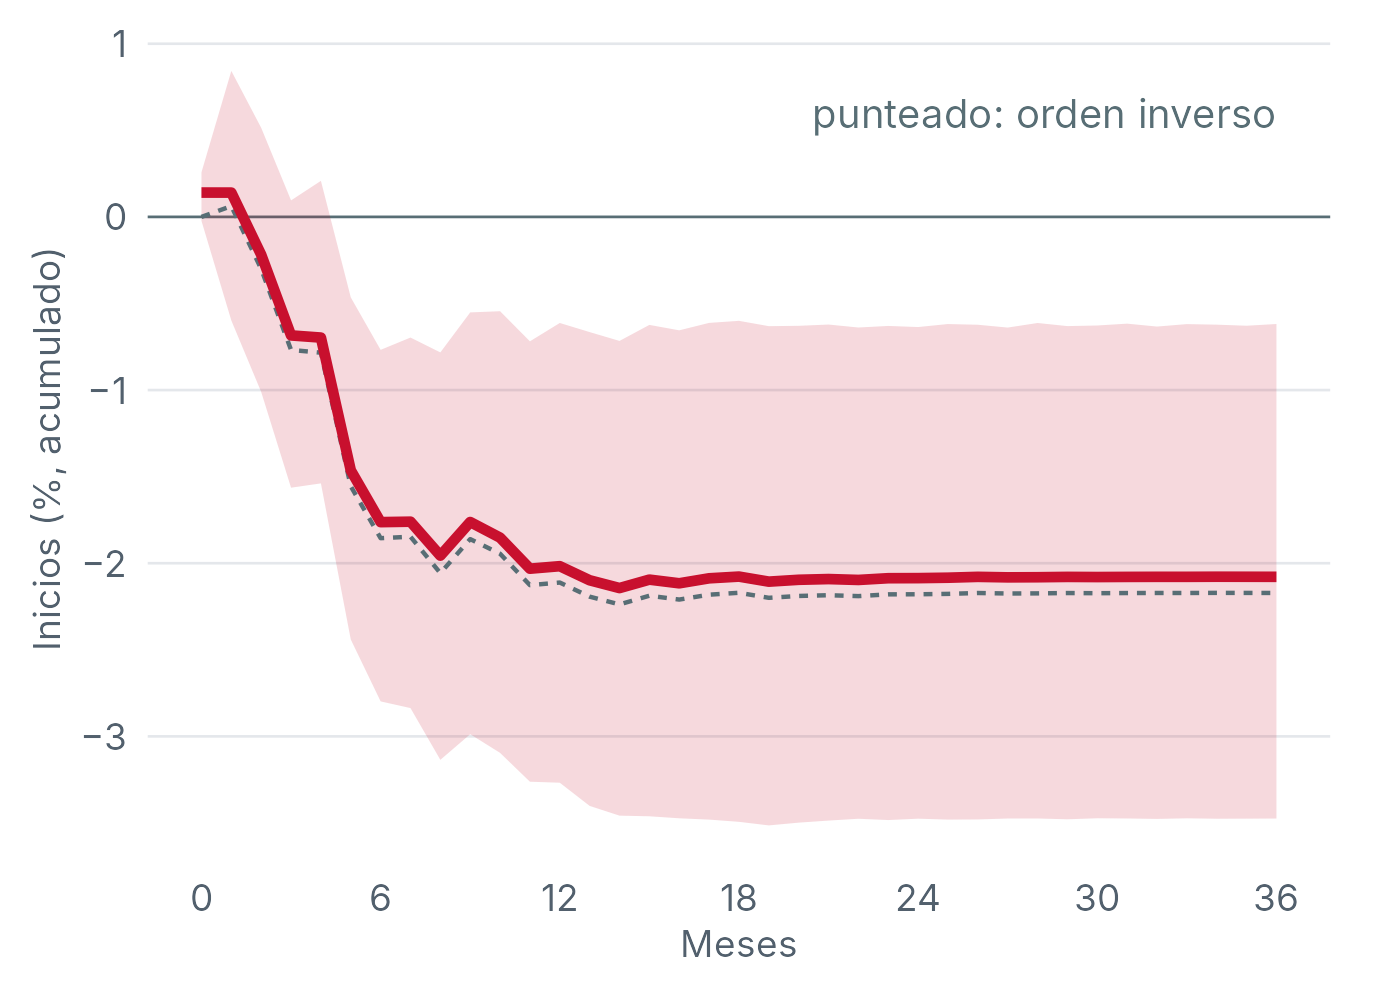
\includegraphics[width=\linewidth,height=0.55\textheight,keepaspectratio]{irf_inicios.png}
    \end{column}
    \begin{column}{0.49\textwidth}
      \centering
      {\small Tasa ante un shock de inicios}\\
      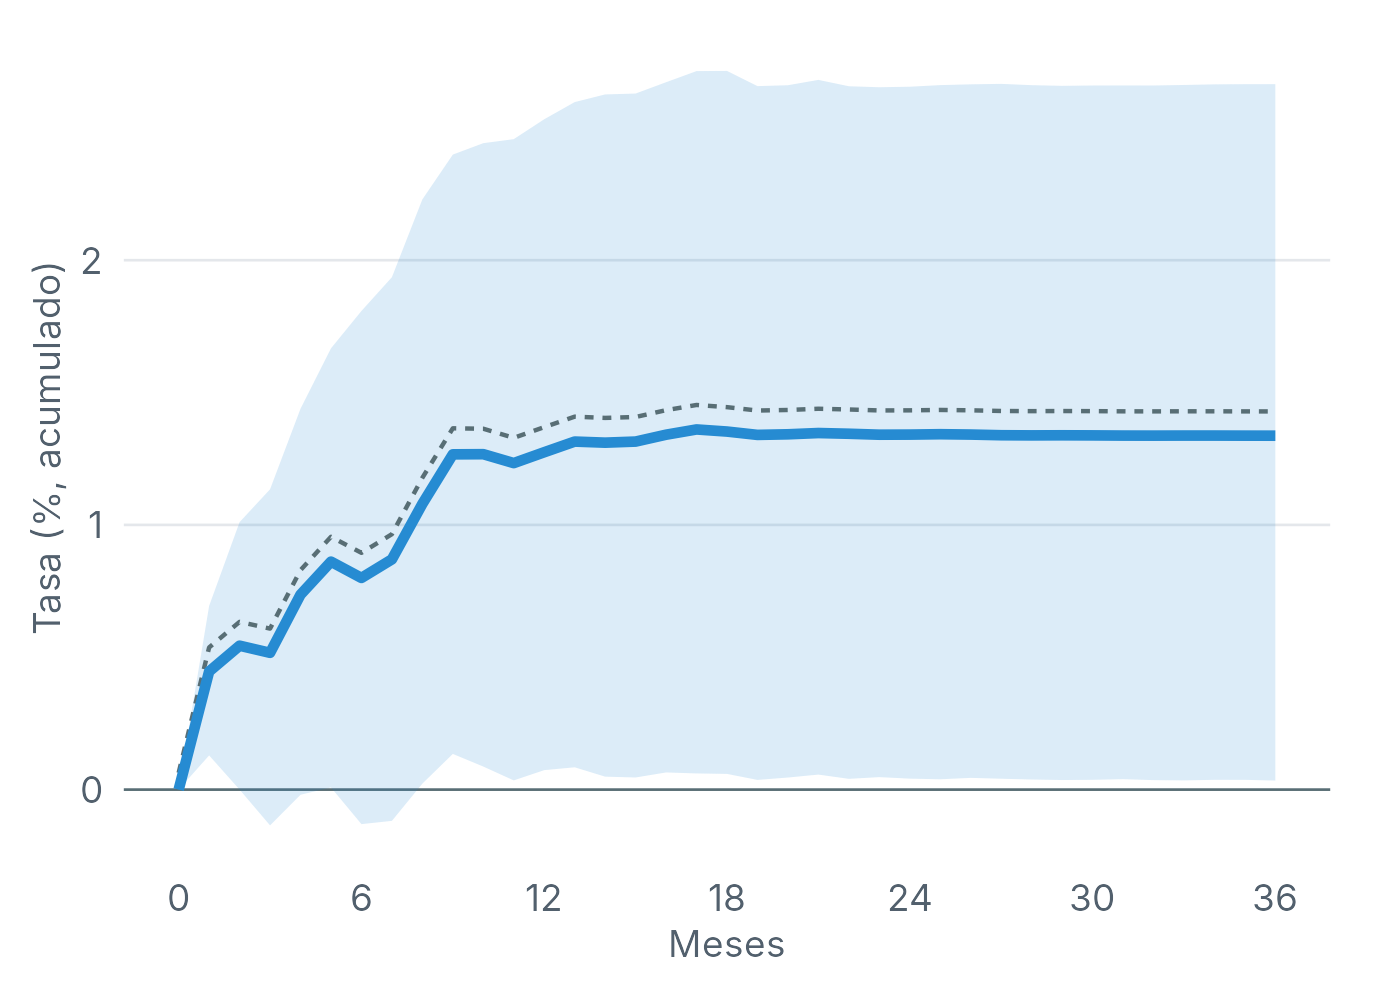
\includegraphics[width=\linewidth,height=0.55\textheight,keepaspectratio]{irf_tasa.png}
    \end{column}
  \end{columns}
  \small
  Shocks de un desvío; bandas por \emph{wild bootstrap}. Con 1 a 3 rezagos el efecto es chico y no significativo, pero esos VAR dejan autocorrelación en los inicios; desde 5 rezagos se parece al de la función de transferencia. El portmanteau conjunto rechaza ($p=0{,}004$).
\end{frame}

\begin{frame}
  \frametitle{Respaldo: la ganancia a lo largo del tiempo}
  \centering
  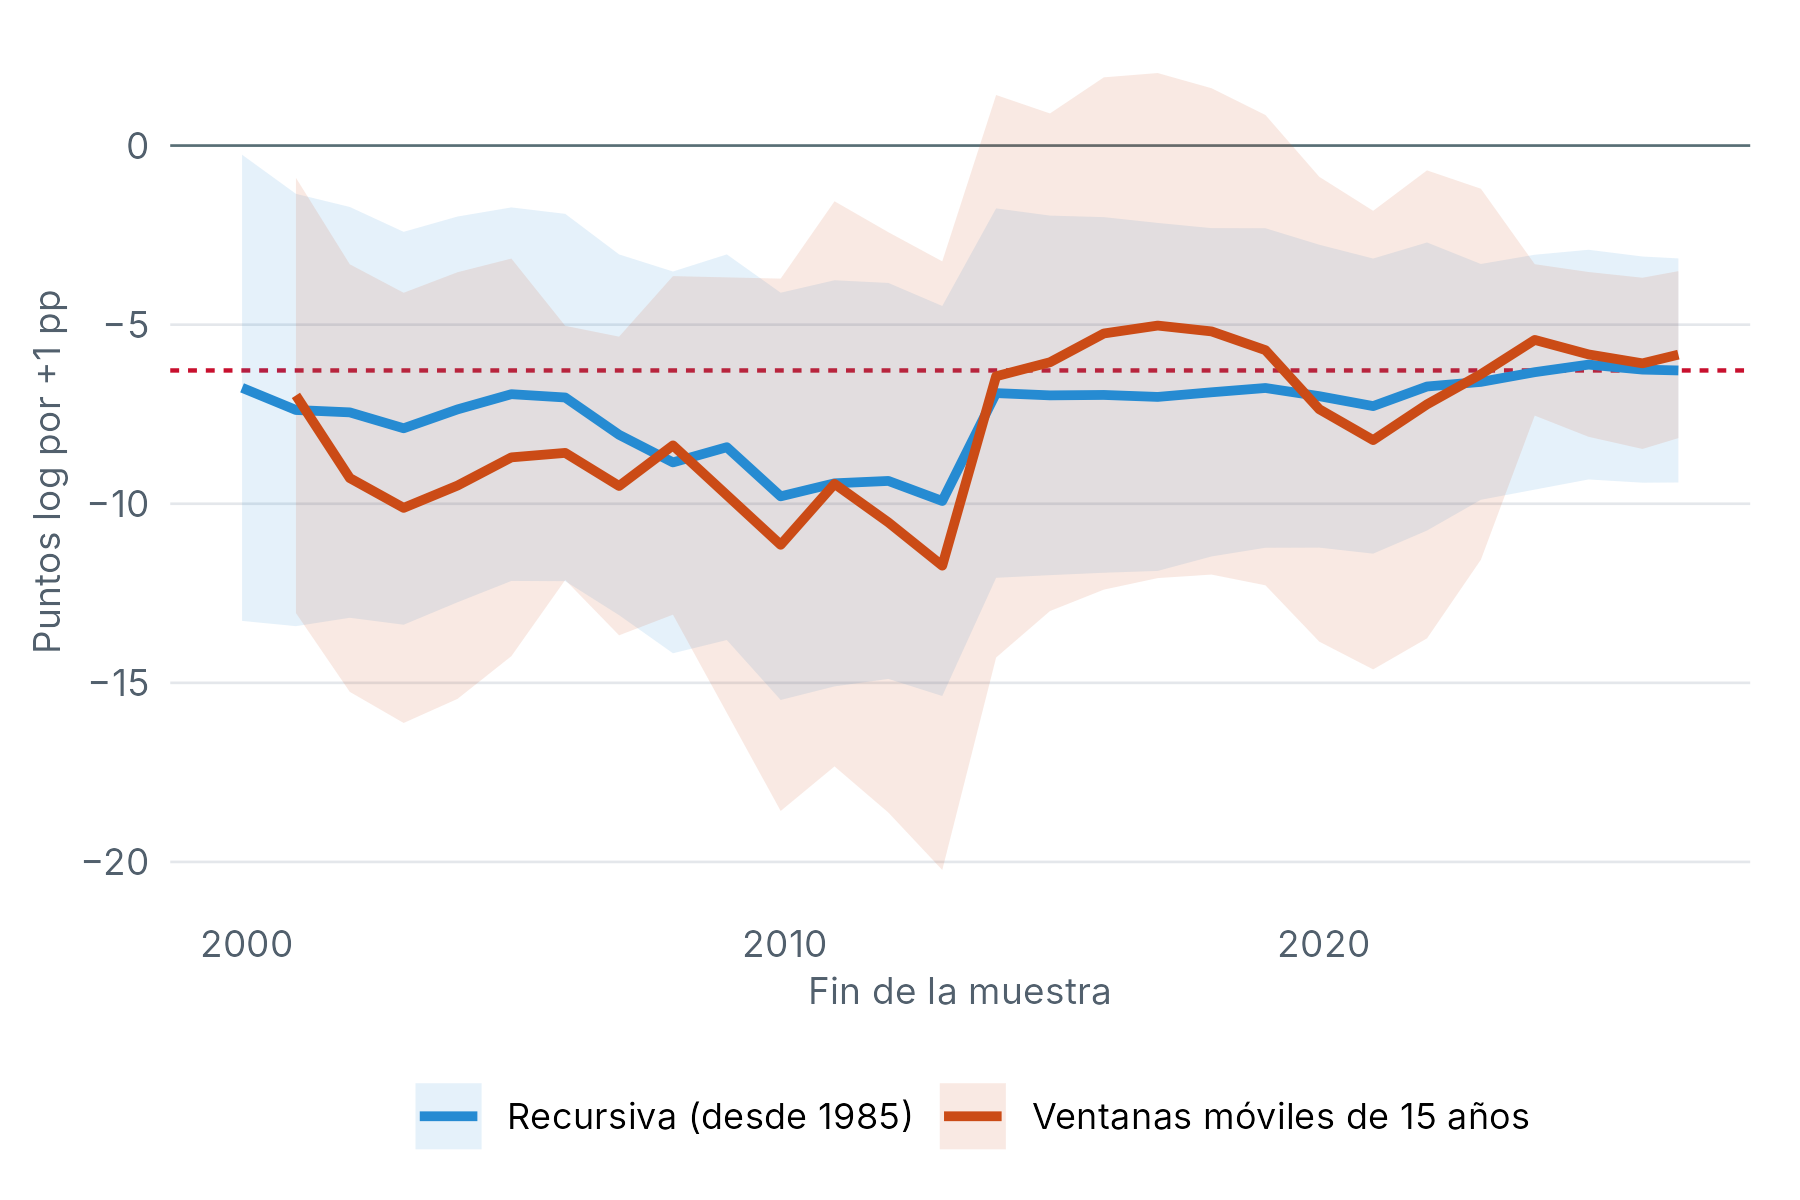
\includegraphics[width=0.85\linewidth,height=0.75\textheight,keepaspectratio]{estab_tiempo.png}

  \small Los valores más negativos corresponden a muestras que terminan entre 2010 y 2013 (colapso inmobiliario).
\end{frame}

\begin{frame}
  \frametitle{Respaldo: permisos, controles e hipótesis no confirmadas}
  \centering\small
  \resizebox{\linewidth}{!}{%
  \begin{tabular}{lll}
    \toprule
    Análisis & Resultado & Lectura \\
    \midrule
    Permisos como \emph{output} & retardo 1 mes; $-8{,}0\%$ por pp & reaccionan antes (ventaja chica en SBC) \\
    + costo de materiales & ganancia $-0{,}42$; $p=0{,}15$ & costos no significativos \\
    + meses de oferta & ganancia $-0{,}38$; $p=0{,}014$ & la oferta es parte del canal \\
    VAR con el bono, tasa primero & $-6{,}5\%$ por pp & exogeneidad por bloques, $p=0{,}26$ \\
    Asimetría (subas vs.\ bajas) & $-0{,}17$ vs.\ $-1{,}02$; $p=0{,}035$ & frágil; falla fuera de la muestra \\
    \emph{Lock-in} (brecha sustituta) & $t=0{,}11$ & no significativo; extrapolación \\
    \bottomrule
  \end{tabular}}
\end{frame}

% ---------- Respaldo: descomposicion anual ----------
\begin{frame}
  \frametitle{Respaldo: la descomposición año por año}
  \centering
  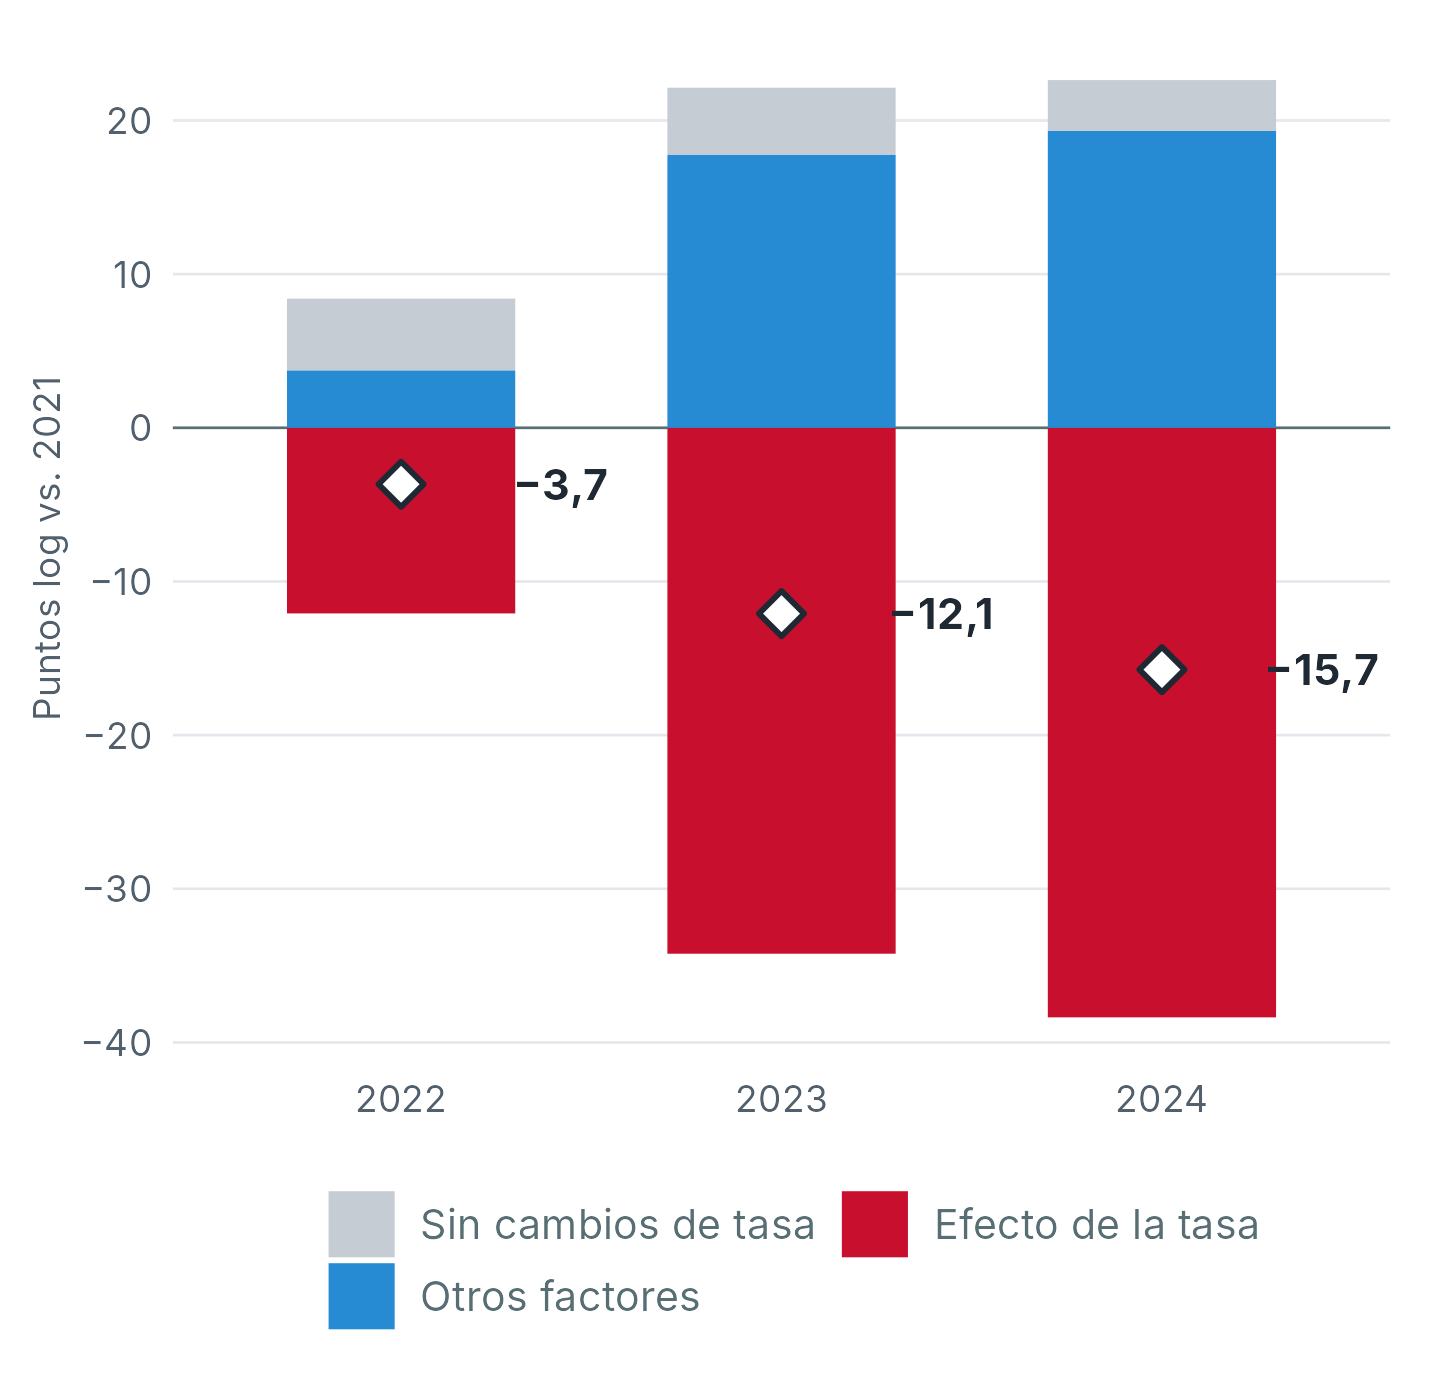
\includegraphics[width=\linewidth,height=0.80\textheight,keepaspectratio]{episodio_barras.png}
\end{frame}

\end{document}
